\documentclass{book}
\usepackage[utf8]{inputenc} %codificación de caracteres que permite tildes
\usepackage[spanish]{babel}

\usepackage{graphicx}
\usepackage{caption}
\usepackage{amssymb}
\usepackage{subcaption}
\usepackage{float}
\graphicspath{ {./Imagenes/} }
\usepackage{listings}

\usepackage{hyperref}
\hypersetup{
	colorlinks=true, %set true if you want colored links
	linktoc=all,     %set to all if you want both sections and subsections linked
	linkcolor=blue,  %choose some color if you want links to stand out
}

\usepackage[
top    = 2cm,
bottom = 2cm,
left   = 1cm,
right  = 1cm]
{geometry}

\newcommand{\dotrule}[1]{%
	\parbox[t]{#1}{\dotfill}}

\title{Resumen Comunicaciones}
\author{LCC - Si tenés alguna contribución pedí el .tex que anda dando vueltas}
\date{$\infty$}

\begin{document}
	\maketitle
	\tableofcontents
	
	\chapter{Unidad I - Introducción}
	
	\section{Hardware de red}
	Existen dos criterios para clasificar redes que se destacan: tecnología de transmisión y escala.
	
	\subsubsection{Tecnología de transmisión}
	Según esta clasificación están: los enlaces de difusión (\textit{broadcast}) y los enlaces punto a punto.
	
	\vspace{3mm}
	Los enlaces punto apunto conectan pares de máquinas. Para ir de un punto a otro en una red conectada por enlaces punto a punto se tienen que visitar máquinas intermedias. El caso en particular en el cual en la red hay solamente un emisor y un receptor se lo conoce como unidifusión (\textit{unicast}).
	
	\vspace{3mm}
	En una red de difusión todas las máquinas en la red comparten un canal de comunicación: quien envía un mensaje especifica a quien se dirige. Todas las máquinas reciben el mensaje pero solo la máquina receptora lo procesa, las demás lo ignoran. Estas redes suelen incorporar una función para enviar paquetes a todos los destinos llamada difusión (\textit{broadcast}) y una para enviar a un subconjunto de máquinas llamada multidifusión (\textit{multicasting}).
	
	\subsubsection{Escala} Según esta clasificación están las PAN, LAN, MAN, WAN e interredes.
	
	\begin{figure}[H]
		\centering
		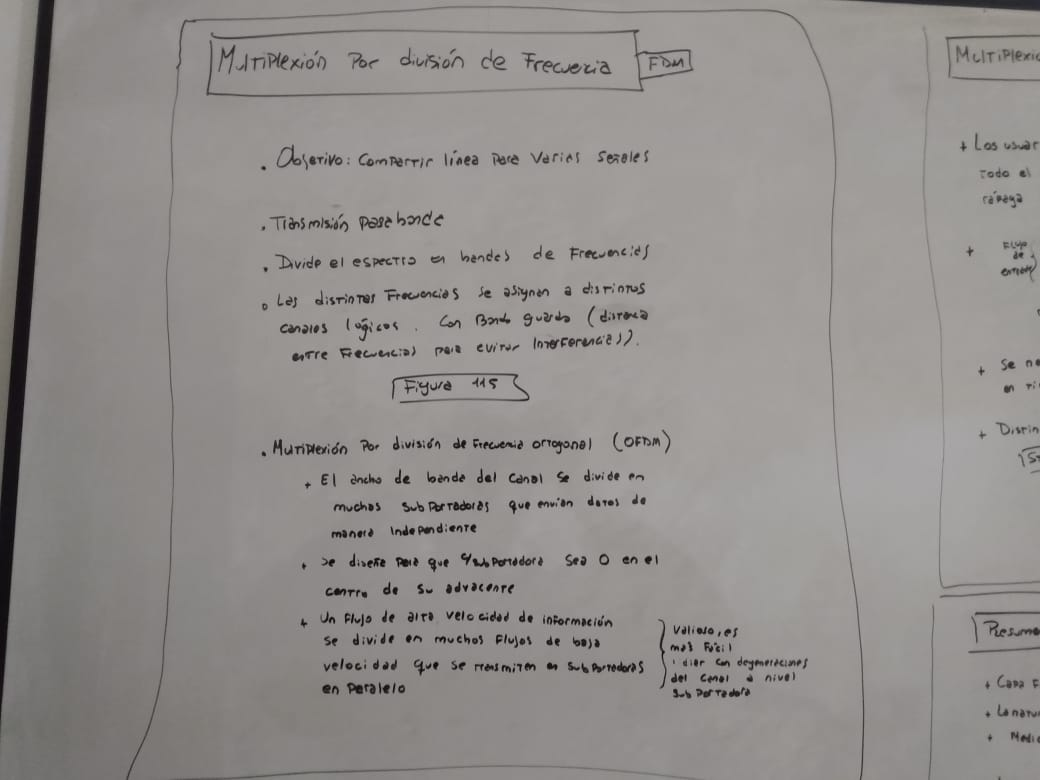
\includegraphics[scale=0.3]{1.png}
	\end{figure}
	
	\pagebreak
	\subsection{PAN - Redes de área personal}
	Las redes de área personal (\textbf{PAN}) permiten a los dispositivos conectarse en el rango de una persona. Ejemplos: conexión entre una computadora y sus periféricos, dispositivos médicos integrados como marcapasos, bombas de insulina o audífonos.
	
	\subsection{LAN - Redes de área local}
	Las redes de área local (\textbf{LAN}) son redes de propiedad privada que operan en edificios, casas, oficinas o fábricas. Se utilizan para conectar computadoras o electrodomésticos con el fin de compartir recursos. Mención especial a \textbf{IoT} (\textit{Internet of Things}).
	
	En la mayoría de las LAN inalámbricas cada computadora se comunica con un punto de acceso (\textbf{AP}) o router inalámbrico el cual permite transmitir paquetes entre computadoras y entre las computadoras e Internet. Existe un estándar para las redes LAN inalámbricas llamado \textbf{IEEE 802.11} o \textbf{WIFI}.
	
	Por otro lado, las tecnologías de transmisión que se usan en LAN alámbricas pueden ser cables de cobre o fibra óptica. Una topología común, ethernet conmutada, incluye a computadoras conectadas a un \textbf{switch} con un enlace punto a punto. El switch se encarga de transmitir paquetes entre las computadoras conectadas a él utilizando la información del paquete. Para estas redes existe un estándar llamado \textbf{IEEE 802.3} o \textbf{Ethernet}.
	
	Otra topología que está en desuso, \textit{Ethernet clásica}, consistía en un solo cable lineal. Una máquina podía transmitir a la vez solamente cuando el canal no estuviera activo. Si ocurría una colisión, las máquinas esperaban un tiempo aleatorio y retransmitían.
	
	Nota: Las redes LAN alámbricas son mejores en redimiento que las inalámbricas ya que es más fácil enviar señales a través cables o fibras que a través del aire. La seguridad favorece a las redes alámbricas pero la conveniencia y el costo a las inalámbricas.
	
	\begin{figure}[H]
		\centering
		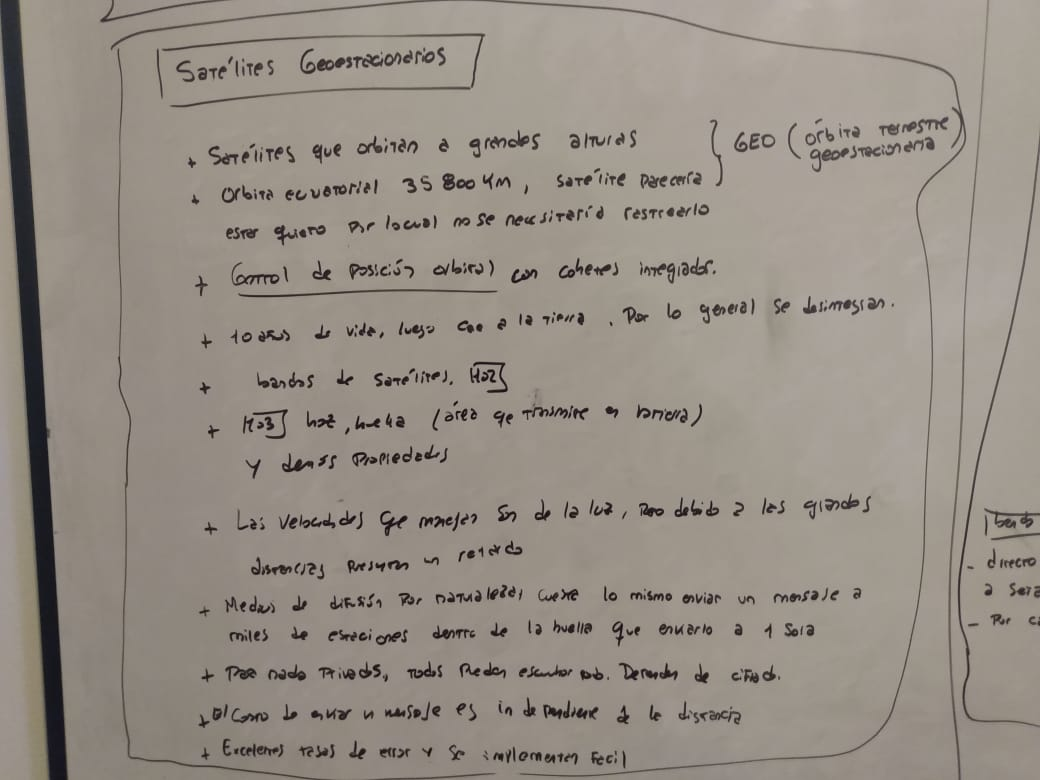
\includegraphics[scale=0.3]{2.png}
	\end{figure}
	
	En muchas empresas ocurre que la distribución del equipo no se corresponde con la estructura de la organización. Es posible dividir una LAN física en varias redes LAN lógicas llamadas \textbf{VLAN} o LAN virtuales de menor tamaño. El switch en estos casos envía los paquetes a cada subconjunto de máquinas pertenecientes a cada LAN virtual.
	
	\subsubsection{Diseño de las redes} Según esta clasificación están los diseños estáticos y los dinámicos.
	
	\vspace{3mm}
	En esta clasificación varía la forma en la que se asigna el canal. Una asignación \textbf{estática} típica consiste el dividir el tiempo en intervalos discretos y utilizar un algoritmo por turno rotatorio (\textit{round-robin}). Esta estrategia desperdicia la capacidad del canal cuando una máquina no tiene nada que enviar en su turno por lo que la mayoría de los sistemas tratan de asignar el canal de forma dinámica.
	
	\vspace{3mm}
	Por otro lado, los métodos de asignación al canal \textbf{dinámicos} pueden ser centralizados o descentralizados. En el centralizado hay una sola entidad que asigna los turnos, como por ejemplo, la estación base en las redes celulares. En el descentralizado cada máquina decide por su cuenta si transmite o no.
	
	\subsection{MAN - Redes de área metropolitana}
	Las redes de área metropolitana (\textbf{MAN}) suelen cubrir ciudades enteras. Ejemplos de éstas son las redes de televisión por cables o el acceso inalámbrico a internet de alta velocidad de estándar \textbf{IEEE 802.16} o \textbf{WiMAX}.
	
	\begin{figure}[H]
		\centering
		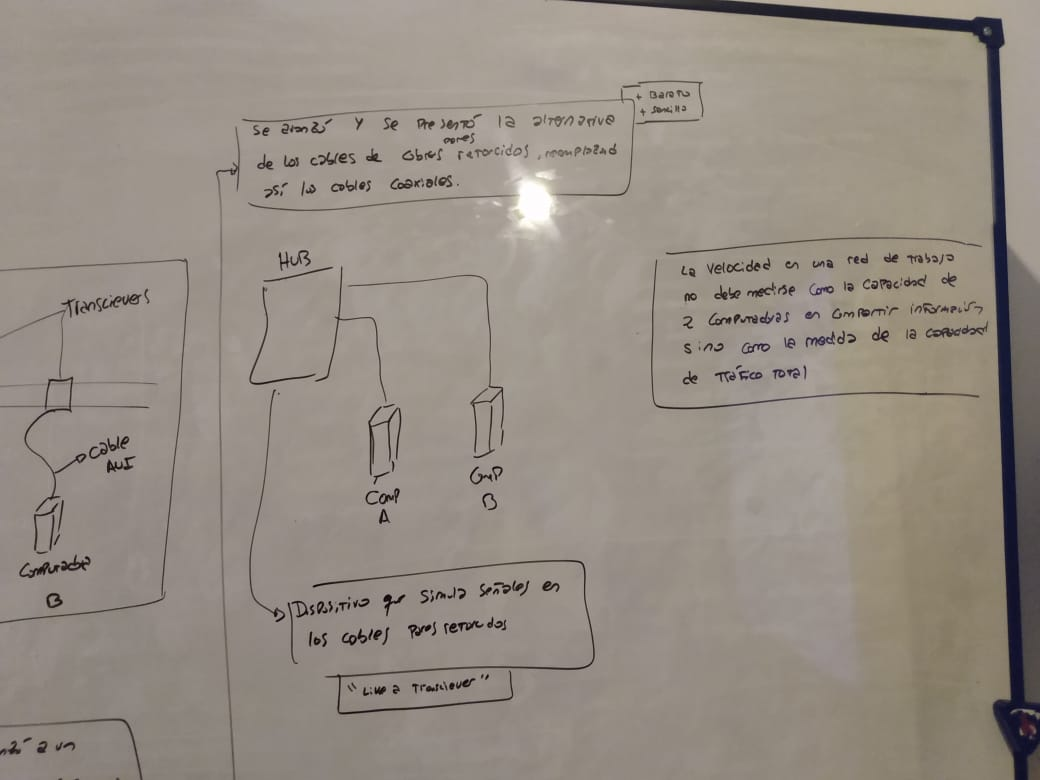
\includegraphics[scale=0.25]{3.png}
	\end{figure}
	
	\subsection{WAN - Redes de área amplia}
	Las redes de área amplia (\textbf{WAN}) abarcan áreas geográfica extensas como países o continentes.
	
	\vspace{3mm}
	Un ejemplo de WAN \textbf{alámbrica} podría ser una empresa con sucursales en diferentes ciudades de Australia. Cada una de eśtas oficinas contiene máquinas destinadas a ejecutar aplicaciones (\textit{hosts}). La parte de la red que conecta a las máquinas se llama \textbf{subred} (de comunicación) y es la encargada de transportar los mensajes.
	
	\begin{figure}[H]
		\centering
		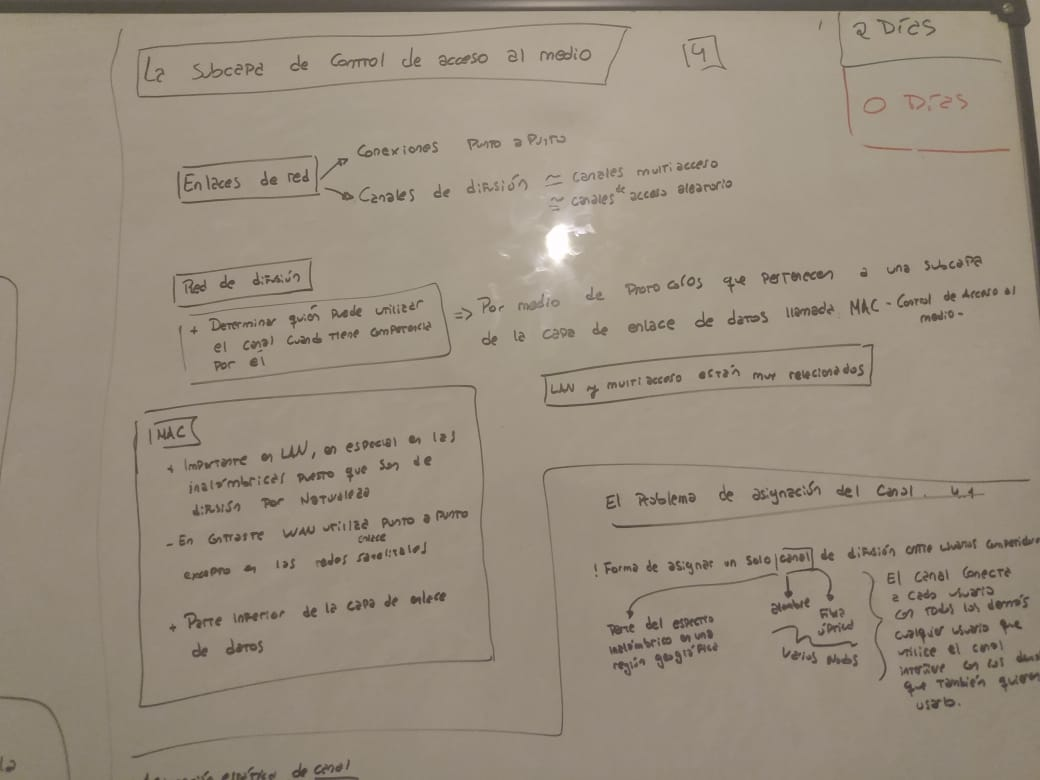
\includegraphics[scale=0.25]{4.png}
	\end{figure}
	
	En la mayoría de las WAN las subredes se componen de líneas de transmisión y y elementos de conmutación. Las líneas de transmisión mueven bits entre máquinas y pueden ser cables de cobre, fibra óptica o inclusive ondas de radio. Las lineas de transmisión se suelen rentar a las compañías de telecomunicaciones.
	
	\vspace{3mm}
	Por otro lado, los elementos de conmutación o switches son computadoras especializadas que conectan dos o más líneas de transmisión. Tuvieron muchos nombres pero ahora se llaman \textbf{routers}.
	
	\vspace{3mm}
	En la WAN, a diferencia de una LAN extensa,
	
	\begin{enumerate}
		\item Los hosts y la subred suelen pertenecen a distintas personas.
		\item Los routers suelen conectar distintos tipos de tecnología.
		\item Lo que se conecta a las subred pueden ser máquinas personales o LAN completas.
	\end{enumerate}
	
	Otro ejemplo de WAN podría incluir una conexión a Internet en vez de la renta de lineas de transmisión. Las conexiones entre sucursales serían enlaces virtuales que utilizan la capacidad subyacente de Internet. A esto se lo denomina \textbf{VPN} o red privada virtual. Las VPN tienen las ventajas y desventajas de la virtualización: son flexibles para reutiizar recursos y fácilmente escalables pero carecen de control real sobre los recursos subyacentes.
	
	\begin{figure}[H]
		\centering
		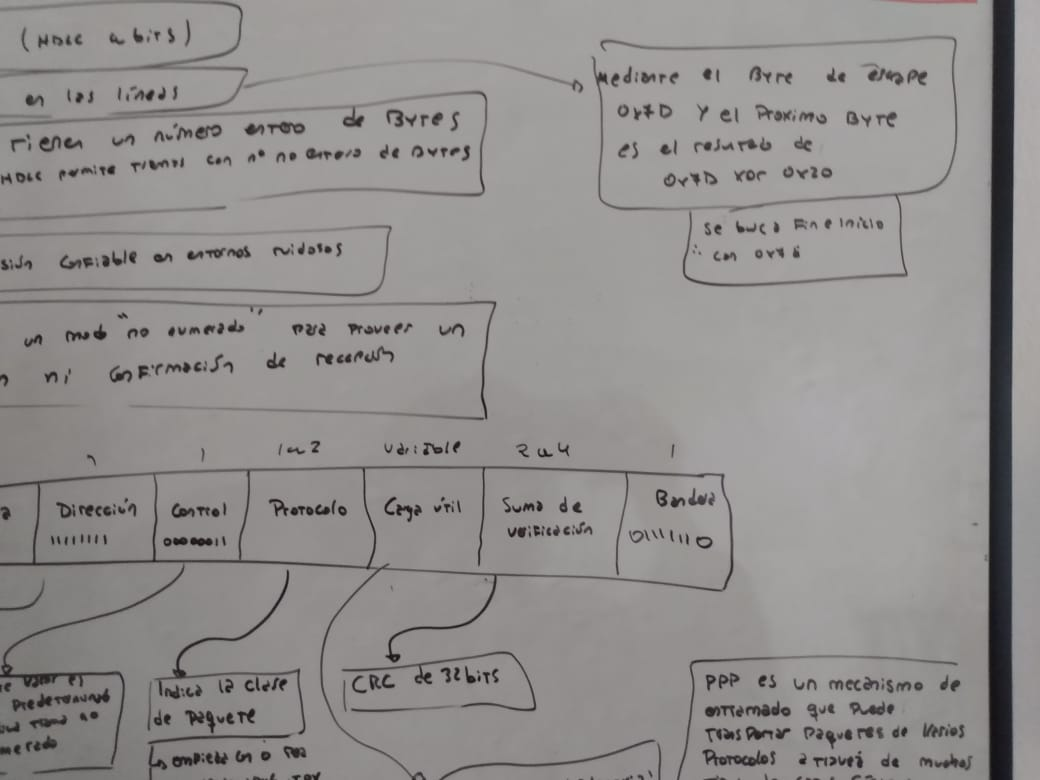
\includegraphics[scale=0.27]{5.png}
	\end{figure}
	
	Un último ejemplo de WAN podría ser que dos empresas coexistan en una subred. Al proveedor de esta subred se lo conoce como \textbf{ISP} (\textit{proveedor de servicion de internet}) y la subred como \textbf{red ISP}. El operador de la subred se conecta con otros clientes siempre que paguen por el servicio. En la red ISP hay muchas líneas de transmisión que conectan varios routers por lo que si dos routers que no están en la misma linea de transmisión desean comunicarse, deberán hacerlo de forma indirecta a través de otros routers, lo cual da lugar a \textbf{algoritmos de enrutamiento}.
	
	\begin{figure}[H]
		\centering
		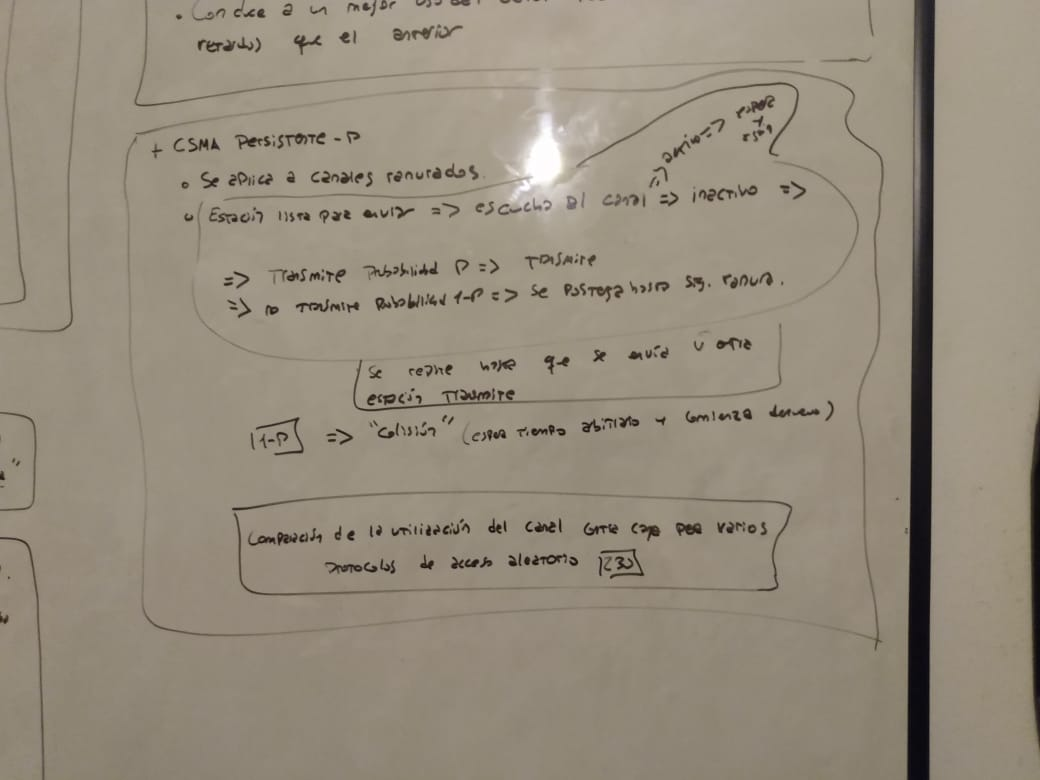
\includegraphics[scale=0.27]{6.png}
	\end{figure}
	
	Otros tipos de redes WAN usan tecnología inalámbrica. En los sistemas de satélites cada computadora en la Tierra tiene una antena a través de la cual es posible enviar y recibir datos de un satélite en órbita. Éstas redes son de difusión por naturaleza.
	
	Un último ejemplo de WAN inalámbrica es el de la telefonía celular. Cada estación base en un sistema celular cubre una distancia mucho mayor que una LAN inalámbrica. Además se conectan entre sí mediante una red troncal que suele ser alámbrica.
	
	\pagebreak
	\subsection{Interredes}
	Por lo general, las personas conectadas a una red se quieren comunicar con personas conectadas en una red distinta por lo que es necesario conectar redes que suelen ser incompatibles. A una colección de redes se la llama interred o internet (con minúscula). La Internet (con mayúscula) es una ejemplo de interred de alcance mundial.
	
	En general, conectar una red LAN y una WAN o dos redes LAN constituye una interred, pero no hay muchos acuerdos en cuanto la terminología. Existen dos reglas prácticas para distinguir las interredes del término más genérico y ambiguo red: 1) Si cada red se construye y mantiene por entidades diferentes. 2) Si la tecnología subyacente es distinta en diferentes partes, por ejemplo difusión y punto a punto o inalámbrica y alámbrica.
	
	En nombre que se le da a la máquina que conecta dos redes distintas es \textbf{puerta de enlace} (\textit{gateway}).
	
	\section{Software de red}
	
	\subsubsection{Jerarquía de protocolos}
	Para reducir la complejidad del diseño, las redes se organizan como una pila de \textbf{capas} o niveles. El número de capas, su nombre, el contenido y la función difieren de red en red. Cada capa ofrece servicios a las capas superiores ocultando los detalles de implementación. Debajo de la primer capa se encuentra el \textbf{medio físico} a través del cual se da la comunicación real.
	
	\vspace{3mm}
	Cuando una capa n en una máquina conversa con una capa n en otra máquina, a las reglas y convenciones utilizadas en esa conversación se las conoce como \textbf{protocolo}. Las entidades que conforman las correspondientes capas en diferentes máquinas se llaman \textbf{iguales} (\textit{peers}).
	
	\vspace{3mm}
	Entre capas adyacentes de una misma máquina hay una \textbf{interfaz} que define operaciones y servicios primitivos que la capa inferior pone a disposición de la capa superior. Las interfaces deben ser limpias y estar bien especificadas y tienen que minimizar la cantidad de información que se pasa entre capas.
	
	\vspace{3mm}
	Al conjunto de capas y protocolos se lo conoce como \textbf{arquitectura de red}. La arquitectura de red es una especificación por lo que no incluye detalles de implementación.
	
	\vspace{3mm}
	Analogía: un filósofo le quiere comunicar a otro filósofo el mensaje "Me gustan los conejos" pero no saben un lenguaje en común. Cada uno contrata a un traductor y a su vez cada uno de ellos contrata a un secretario para enviar el mensaje.
	
	El mensaje recorre el primer filósofo, el primer traductor, el primer secretario, el segundo secretario, el segundo traductor y finalmente llega al segundo filósofo. Pero se puede pensar que virtualmente, se comunican capa a capa (protocolo). Cada protocolo es independiente de los demás siempre que no se cambien las interfaces: los traductores pueden cambiar el idioma al cual traducen y los secretarios pueden cambiar el medio por el cual envían el mensaje.
	
	\begin{figure}[H]
		\centering
		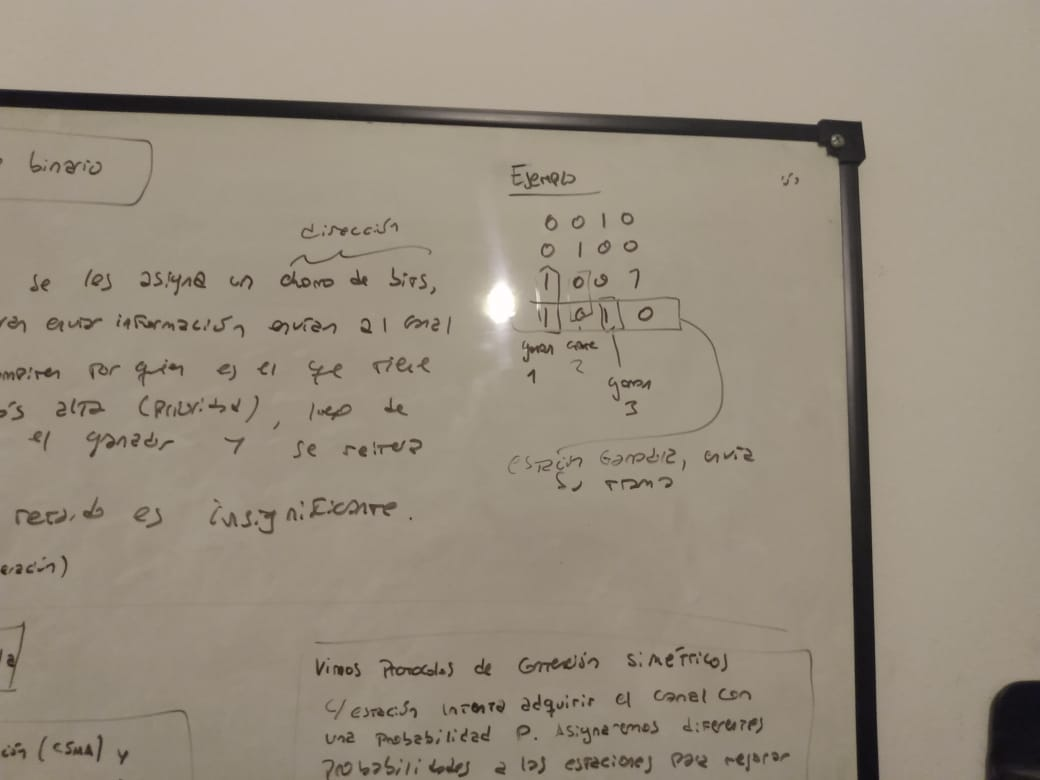
\includegraphics[scale=0.4]{7.png}
	\end{figure}
	
	Técnicamente hablando, cada protocolo de capa coloca un encabezado que solamente puede remover el mismo (en otra máquina). Este encabezado puede contener información de control como números de secuencia en caso de fragmentación, tamaños o tiempos. La capa inferior, además de agregar un encabezado agrega un terminador para su transmisión física. Ningún encabezado de las capas inferiores a n pasa a la capa n.
	
	\begin{figure}[H]
		\centering
		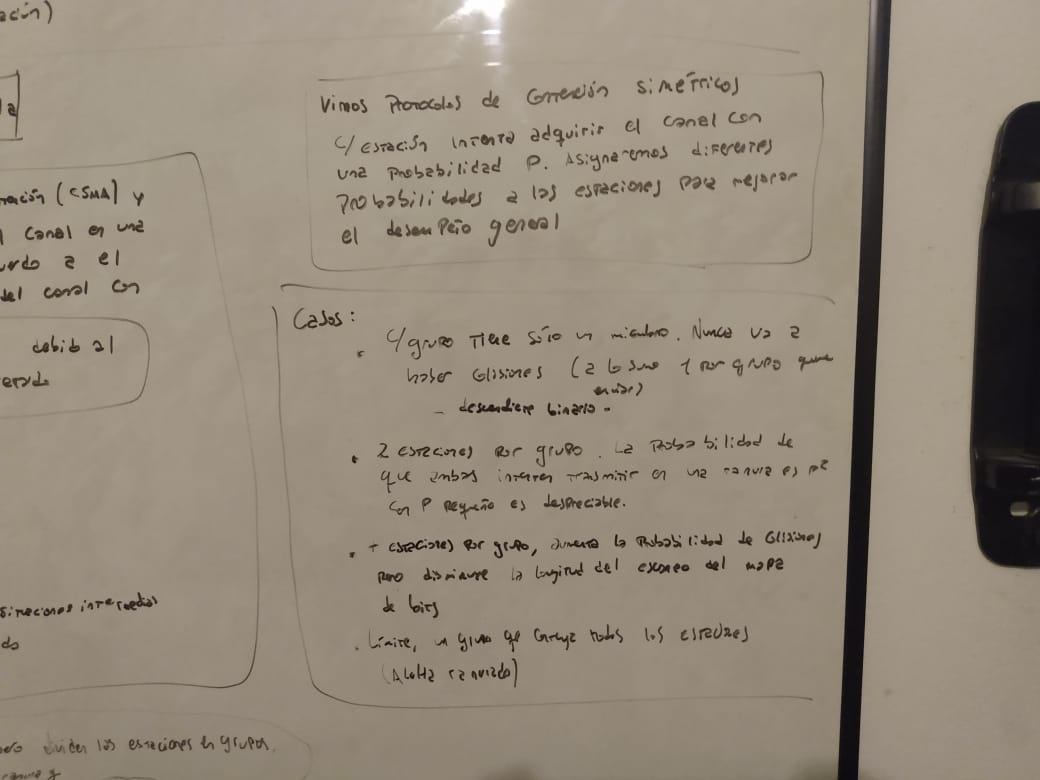
\includegraphics[scale=0.37]{8.png}
	\end{figure}
	
	\subsubsection{Diseño de capas}
	Algunos aspectos clave para el diseño de capas son
	
	\begin{itemize}
		\item confiabilidad: la red debe operar correctamente aunque esté formada por una colección de componentes poco confiables.
		
		\subitem - Un mecanismo para detectar errores es la \textbf{detección de errores}. Cuando se detecta un error se puede o bien retransmitir o bien recuperar el mensaje a través de la \textbf{corrección de errores} a partir de información redundante agregada.
		
		\subitem - Para encontrar una ruta funcional para enviar mensajes se utilizan algoritmos de enrutamiento.
		
		\item evolución de la red: para redes cada vez más grandes con diseños más complejos resulta clave la abstracción y el encapsulamiento de los protocolos en las capas.
		
		\subitem - direccionamiento o nombramiento: cada capa debe poder identificar a emisores y receptores involucrados en un mensaje.
		
		\subitem - interconexión de redes o internetworking: diferentes redes tienen diferentes limitaciones. Lo cual en muchos casos induce a el desensamblaje, la transmisión y el posterior ensamblaje de los mensajes.
		\subsubitem * Algunas preservan el orden de los mensajes y otras no
		\subsubitem * Muchas tienen tamaño máximo de mensajes diferentes.
		
		\subitem - escalabilidad: pueden surgir problemas de tráfico, escasez de nombres, etc.
		\item asignación de recursos: se deben dividir de forma de que no interfieran con el host. 
		\subitem - Un problema común llamado \textbf{control de flujo} es evitar que un emisor rápido envíe más de lo que el receptor puede recibir. 
		\subitem - La \textbf{congestión} es otro problema que hace que las redes se sobrecarguen.
		\subitem - A veces la puntualidad de la entrega es importante (streaming por ejemplo). La calidad de servicio o \textbf{QoS} es el nombre que se le da a los mecanismos que reconcilian estas demandas competitivas.
		
		\item confidencialidad: los mecanismos de autenticación y de integridad tratan de evitar amenazas a la red.
	\end{itemize}
	
	\subsubsection{Servicio orientado a la conexión y servicio sin conexión - Confiabilidad}
	Las capas pueden ofrecer servicios orientados a la conexión o sin conexión.
	
	\vspace{3mm}
	En los servicios \textbf{orientados a la conexión} el usuario primero establece la conexión, luego la utiliza y luego la libera. Esencialmente la conexión funciona como un tubo: el emisor mete bits en un tubo y el receptor los recibe. Por lo general, el orden de los mensajes se preserva. Es común que al establecer la conexión, emisor y receptor negocien parámetros como tamaño del mensaje, calidad requerida del servicio, etc. Ejemplo: sistema telefónico.
	
	\vspace{3mm}
	En el servicio \textbf{sin conexión} cada mensaje lleva la dirección del destino completa y se enruta hacia los nodos internos del sistema de forma independiente a los otros mensajes. El mensaje puede llegar fuera de orden o no llegar Ej: código postal.
	
	\vspace{3mm}
	En las implementaciones de los servicios \textbf{confiables} el receptor suele confirmar que recibió el mensaje. El proceso de confirmación de recepción introduce sobrecarga y retardos que a veces no son deseables. Un ejemplo de servicio confiable es el envío de archivo: los bits deben llegar por completo y en el mismo orden.
	
	\vspace{3mm}
	Los servicios orientados a la conexión confiables tienen dos variaciones: \textbf{secuencia de mensajes} (Se conservan los límites de los mensajes) y \textbf{flujo de bytes} (el flujo no tiene límites y no se pueden reconstruir los mensajes originales por separado). Ejemplo de secuencia de mensajes: composición de páginas de un libro. Ejemplo de flujo de bytes: descarga de una película.
	
	\vspace{3mm}
	A los servicios sin conexión no confiables se lo denomina servicio de \textbf{datagramas}. Ejemplo: envío de telegramas. Cuando son sin conexión pero confiables se puede usar el servicio de \textbf{datagramas con confirmación de recepción}. Ejemplo: mensajería de texto de teléfonos móviles.
	
	\begin{figure}[H]
		\centering
		\includegraphics[scale=0.3]{9.png}
	\end{figure}
	
	\begin{table}[H]
		\centering
		\begin{tabular}{|c|c|c|}
			\hline
			&Orientado a la conexión&Sin conexión\\
			\hline
			Confiable&TCP&Mensajes de texto\\
			\hline
			No confiable&voz sobre IP (se introduce ruido)&IP - UDP - Iot (sensores en el campo,\\
			&videollamadas (se pierden píxeles)& sensores de estacionamiento)\\
			\hline
		\end{tabular}
		\caption{Ejemplos vistos en clase}
	\end{table}
	
	\subsection{Modelos de referencia}
	\paragraph{Modelo OSI}
	La fortaleza del OSI es el modelo en sí (excepto por las capas de presentación y sesión)
	\begin{figure}[H]
		\centering
		\includegraphics[scale=0.35]{10.png}
	\end{figure}
	
	\pagebreak
	\subsubsection{Modelo TCP/IP}
	La fortaleza del TCP/IP son los protocolos
	\begin{figure}[H]
		\centering
		\includegraphics[scale=0.25]{11.png}
	\end{figure}
	
	\begin{figure}[H]
		\centering
		\includegraphics[scale=0.25]{12.png}
	\end{figure}
	\paragraph{Modelo Híbrido}
	El que vamos a estudiar (híbrido), se ve así
	
	\begin{figure}[H]
		\centering
		\includegraphics[scale=0.2]{13.png}
	\end{figure}
	
	O más específicamente, así
	
	\begin{figure}[H]
		\centering
		\begin{subfigure}{0.4\textwidth}
			\centering
			\includegraphics[scale=0.15]{36.png}
		\end{subfigure}
		\qquad
		\begin{subfigure}{0.4\textwidth}
			\centering
			\includegraphics[scale=0.15]{37.png}
		\end{subfigure}
	\end{figure}
	
	\begin{itemize}
		\item La capa \textbf{física} especifica cómo transmitir bits a través de diferentes medios
		\item La capa de \textbf{enlace} trata sobre cómo enviar mensajes de longitud finita entre computadoras conectadas de manera directa con niveles específicos de confiabilidad. Ethernet y 802.11 son ejemplos de protocolos en esta capa.
		\item La capa de \textbf{red} se encarga de combinar enlaces múltiples en redes y redes de redes en interredes. Es esta capa entra en juego la tarea de buscar la ruta por la cual se envían paquetes. IP es el principal protocolo de esta capa.
		\item La capa de \textbf{transporte} fortalece las garantías de entrega en la anterior capa y provee abstracciones en la entrega como un flujo de bytes confiable que coincida con las necesidades de las distintas aplicaciones. TCP es un ejemplo de protocolo de esta capa
		\item La capa de \textbf{aplicación} contiene programas que hacen uso de la red. DNS es un ejemplo de programa de soporte de esta capa.
	\end{itemize}
	
	Extra: leer críticas particulares de los modelos por separado.
	Historia de la Internet (ARPAnet)
	
	\chapter{Unidad II - Capa física}
	
	\section{Base teórica}
	Mediante la variación de alguna propiedad física como el voltaje o la corriente es posible transmitir información a través de cables. Si representamos la propiedad física en función del tiempo $f(t)$ podemos modelar el comportamiento de la señal y analizarlo matemáticamente.
	
	\subsection{Análisis de Fourier}
	Fourier demostró que cualquier función periódica de comportamiento razonable, $g(t)$ con período T, se puede construir como la suma de un número (posiblemente infinito) de senos y cosenos
	
	\begin{equation}
	g(t) = \frac{1}{2}c + \sum_{n = 1}^{\infty} a_{n} \sen (2\pi n f t) + \sum_{n = 1}^{\infty} b_{n} \cos (2\pi n f t)
	\end{equation}
	
	en donde $f = \frac{1}{T}$ es la frecuencia fundamental, $a_{n}$ y $b{n}$ son las amplitudes del seno y coseno del n-ésimo armónico y $c$ es una constante. A esa descomposición se la llama serie de Fourier. Extra: con algunos cálculos se pueden obtener $a_{n}$, $b_{n}$ y $c$ en función de $g$.
	
	Con este teorema y conociendo el período, podemos reconstruir la función original a partir de una suma de senos y cosenos. Además, se pueden pensar a las señales de datos de duración finita como infinitas repitiendo períodos completos.
	
	\subsection{Ancho de banda limitado}
	En la comunicación de datos, los canales reales afectan a las señales. La transmisión del carácter ASCII 'b' codificado en un byte:
	
	\begin{figure}[H]
		\centering
		\includegraphics[scale=0.5]{14.png}
	\end{figure}
	
	Durante el envío de señales se pierde potencia en el proceso. Si todos los componentes de Fourier disminuyeran en la misma proporción no habría distorsión (solo cambio de amplitud), pero eso no ocurre (los componentes de Fourier se disminuyen en distinto grado y generan distorsión).
	
	\vspace{3mm}
	El rango de frecuencia que se transmite sin atenuación considerable se llama \textbf{ancho de banda}. El ancho de banda es una propiedad física del medio (construcción, grosor, longitud). Las señales que van desde una frecuencia 0 a una máxima se llaman \textbf{banda-base}, las que se desplazan para superar ese máximo \textbf{pasa-banda}.
	
	\vspace{3mm}	
	Si el medio tuviera un ancho de banda que solamente permitiera pasar las frecuencias más bajas, no podríamos decodificar el carácter 'b' en el receptor (figura a-d). A partir de los 8 armónicos se recibe una señal con la suficiente fidelidad como para reconstruir el carácter 'b', más sería un desperdicio.
	
	\vspace{3mm}
	Si tenemos una tasa de bits de b bits/seg, el tiempo para enviar 8 bits secuencialmente (carácter 'b') es de 8/b segundos. Más aún, la frecuencia del primer armónico (portadora) es b/8 Hz.
	
	\vspace{3mm}
	En general, al limitar el ancho de banda, se limita la tasa de datos, incluso para canales libres de ruido. Esta es la principal motivación para codificar más información en un símbolo (unidad de información que hasta ahora podía ser 0 o 1).
	
	\pagebreak
	\subsection{Tasa de datos máxima de un canal}
	Incluso un canal perfecto tiene una capacidad de transmisión finita.
	
	\vspace{3mm}
	Teorema de Nyquist: Si se pasa una señal cualquiera a través de un filtro pasa-bajas con un ancho de banda B, la señal filtrada se puede reconstruir por completo tomando 2B muestras por segundo (suponiendo 2 niveles). Si la señal consiste de V niveles discretos,
	
	\begin{equation}
	TBM = 2B\log_{2} V
	\end{equation}
	
	Este resultado no es directamente aplicable ya que en la vida real hay siempre ruido presente (térmico, producido por el movimiento de las moléculas). Entre más niveles haya, más va a afectar el ruido térmico. La cantidad de ruido térmico se mide en base a la relación entre la potencia de la señal y la potencia del ruido, llamada \textbf{SNR} (\textit{signal-to-noise} ratio).\footnote{Más potencia, más ruido térmico.} Si S es la potencia de la señal y N la del ruido, la SNR es $\frac{S}{N}$ y se suele expresar en escala logarítmica (no lineal) como la cantidad $10 \log _{10}\frac{S}{N}$ de unidad decibel (dB).
	
	\vspace{3mm}
	Teorema de Shannon: la tasa de datos máxima (o capacidad) de un canal ruidoso cuyo ancho de banda es BHz y cuya relación señal a ruido es S/N está dada por:
	
	\begin{equation}
	TBM = B\log_{2}(1 + S/N)
	\end{equation}
	
	\section{Medios de transmisión}
	Cada medio tiene su propio nicho en términos de ancho de banda, retardo, costo y facilidad de instalación y mantenimiento.
	
	\subsubsection{Sentido de la comunicación}
	\begin{itemize}
		\item simplex: un solo sentido
		\item half-duplex: bidireccional, un sentido a la vez
		\item full-duplex: bidireccional, dos sentidos a la vez
	\end{itemize}
	
	\subsection{Medios de transmisión guiados}
	
	\subsubsection{Medios removibles}
	Una de las formas más simples de transportar información es almacenarla en medios removibles como DVD regrabables, transportarlos físicamente y leer la información en destino.
	
	\begin{center}
		\textit{Nunca subestimes el ancho de banda de una camioneta repleta de DVDs que viaja a toda velocidad por autopista.}
	\end{center}
	
	\subsubsection{Par trenzado}
	Un par trenzado consta de dos cables de cobre aislados de aprox. 1mm de grosor. Los cables están trenzados de forma helicoidal para cancelar las ondas que irradian (antena simple). La señal se transmite como la diferencia de voltaje entre los cables del par (el ruido externo afecta a ambos cables por igual).
	
	\vspace{3mm}
	El par trenzado puede transmitir a lo largo de varios kilómetros sin necesidad de amplificación, pero en distancias mayores se necesitan repetidores. Además, cuando muchos pares trenzados se tienden en paralelo necesitan de una funda protectora debido a la interferencia que generan.
	
	\vspace{3mm}
	Este cable permite transmitir información analógica (sistema telefónico tradicional) o digital (internet antiguamente). Su ancho de banda depende de la construcción del cable y de la distancia que recorre.
	
	\vspace{3mm}
	Los pares trenzados se suelen agrupar de a 4 pares con un aislante. A este arreglo se lo llama cable UTP (par trenzado sin blindaje, \textit{unshielded twisted pair})y distintos estándares LAN lo usan de diferentes maneras (aprovechando 2 cables o los 4 para llegar a velocidades más altas).
	
	\subsubsection{Cable coaxial}
	Este cable tiene mejor blindaje y ancho de banda que los pares trenzados, por lo que puede abarcar mayores distancias a velocidades más altas. Consiste en un alambre de cobre rígido de núcleo, rodeado de aislante, forrado con un conductor cilíndrico y cubierto por una funda. Se usaban para las lineas de larga distancia en el sistema telefónico o para redes de área metropolitana pero ahora están prácticamente es desuso.
	
	\subsubsection{Fibra Óptica}
	La fibra óptica se utiliza para la transmisión de larga distancia en las redes troncales, las redes LAN de alta velocidad y el acceso a internet de alta velocidad FTTH (fibra para el hogar, \textit{fiber to the home}).
	
	\vspace{3mm}
	Este sistema de transmisión optico se compone de una fuente de luz (láser semiconductor o LED), un medio de transmisión y un detector (es unidireccional!). Por convención, la luz indica un 1 y la ausencia de luz un 0. El medio de transmisión es una fibra de vidrio ultradelgada cuyo indice de refracción es tal que el haz de luz rebota con un ángulo mayor al crítico y se mantiene por completo dentro de la fibra.
	
	\vspace{3mm}
	Una fibra en donde los rayos rebotan con distinto ángulo (todos mayores al crítico) se llama \textbf{fibra multimodal}. En contraste, si una fibra tiene prácticamente el tamaño de un haz de luz, la luz se propaga en línea recta y a esta \textbf{fibra} se la llama \textbf{monomodo}. Éstas últimas se usan para distancias más largas (intercontinentales).
	
	\vspace{3mm}
	La fibra óptica hace que las computadoras sean las lentas en el proceso de comunicación: proveen un ancho de banda que es en la práctica infinito.
	
	\paragraph{Construcción y mantenimiento}
	Los cables de fibra óptica son similares a los coaxiales excepto por el trenzado. En el centro se encuentra el núcleo de vidrio (del tamaño de un cabello en la multimodo o más pequeño en la monomodo), rodeado de un revestimiento de vidrio (con distinto índice de refracción). Por lo general las fibras se agrupan en haces con una funda exterior.
	
	\vspace{3mm}
	La fibra es más costosa de instalar que el cable de cobre debido a que en muchos casos se hace bajo tierra o en el fondo marino. Se pueden interconectar mediante 
	
	\begin{itemize}
		\item conectores con clavijas de fibra(introducen atenuación pero facilitan la reconfiguración),
		\item empalme mecánico (se tardan 5 minutos en empalmar y se pierden 10\% de la luz) o
		\item fusión (atenuación mínima)
	\end{itemize}
	
	Las fibras ópticas no se ven afectadas por las sobrecargas de energía, la interferencia electromagnética ni por los cortes en el suministro de energía. Pero sí se dañan si se las dobla.
	
	\subsubsection{Resumen}
	\begin{table}[H]
		\centering
		\begin{tabular}{|c|c|c|c|}
			\hline
			Medio de transmisión&Ancho de banda&Retardo&Costo de instalación y mantenimiento\\
			\hline
			\hline
			Medios removibles&Excelente&Alto (horas)&Bajo (compra DVD)\\
			\hline
			Par trenzado&Bueno&Medio&Bajo (repetidores cada 5k, aislante)\\
			\hline
			Cable coaxial&Muy bueno&Bajo&Bajo\\
			\hline
			Fibra óptica&$\infty$&Muy bajo&Muy bajo (repetidores 50k multi- 250k mono, material liviano)\\
			\hline
		\end{tabular}
	\end{table}
	
	\pagebreak
	\subsection{Medios de transmisión no guiados - transmisión inalámbrica}
	Suelen ser prácticos cuando no se puede acceder físicamente a una zona intermedia para la comunicación, para simplificar cableado y/o para usuarixs móviles.
	
	\subsubsection{Base teórica}
	Cuando los electrones se excitan, crean ondas electromagnéticas que se pueden propagar por el espacio. El número de oscilaciones por segundo de una onda es su frecuencia $f$ (Hz), la distancia entre dos máximos (o mínimos) consecutivos se llama longitud de onda $\lambda$ (m).
	
	\vspace{3mm}
	Al conectar una antena a un circuito eléctrico, las ondas se pueden difundir y un receptor las puede captar a una cierta distancia. Toda la comunicación inalámbrica se basa en este principio. La velocidad de la luz $c$ (m/s) es el máximo teórico de velocidad de propagación.
	
	\begin{figure}[H]
		\centering
		\includegraphics[scale=0.4]{15.png}
	\end{figure}
	
	Dentro del espectro magnético (figura) se puede ver la porción que va desde radio hasta luz visible para transferir información. Las restantes serían perjudiciales para la salud de las personas. Las ondas pueden llevar información si se las modula y luego demodula por amplitud, frecuencia o fase. Los nombres LF, MF, HF, VHF, UHF (\textit{low}, \textit{medium}, \textit{high}, \textit{very high} y \textit{ultra high} frecuency) hacen referencia a nombres oficiales de ciertas bandas de frecuencias acuñadas por la ITU (unión internacional de telecomunicaciones, \textit{International Telecommunications Union}).
	
	\vspace{3mm}
	Por lo general, las transmisiones utilizan una banda de frecuencia estrecha para usar el espectro con eficiencia y obtener tasas de datos razonables al transmitir suficiente potencia. En el caso que no utilicen una banda estrecha, existen 5 variaciones / técnicas:
	
	\begin{itemize}
		\item FHSS - espectro disperso con salto de frecuencia, \textit{Frequency-Hopping Spread Spectrum}: el ancho de banda se divide en ranuras de frecuencia disjuntas. Permite obtener anchos de banda de al menos un orden de magnitud mayor que los anchos de banda permitidos por DSSS (sig item). El transmisor salta de frecuencia en frecuencia cientos de veces por segundo. Se suele utilizar en comunicación militar o en casos comerciales como Bluetooth o 802.11 (WIFI)
		
		\item DSSS - espectro disperso de secuencia directa, \textit{Direct Sequence Spread Spectrum}: Las señales suelen recibir códigos (por ejemplo CDMA, \textit{code division multiple access} del siguiente capítulo). La secuencia de bits utilizada para modular los bits se conoce como \textbf{secuencia de Barker}. Forma la base de la telefonía móvil 3G y es parte de algunos sistemas GPS.
		
		\item UWB - Banda ultra ancha, \textit{ultra wide band}: se envían una serie de pulsos rápidos, los cuales varían sus posiciones para comunicar información. Se utilizan en redes PAN inalámbricas, para tomar imágenes a través de objetos sólidos y como parte de sistemas de ubicación precisos.
		
		\item MIMO - múltiple entrada múltiple salida, \textit{Multiple-input Multiple-output}: utiliza varias antenas (transmisores y receptores) lo cual genera subcanales equivalentes paralelos e independientes (se transmite a mayor velocidad). Aprovecha las ventajas del fenómeno de ondas \textbf{multiruta} en el cual la señal rebota en paredes y techos.
		
		\item MUMIMO - MIMO de múltiple usuario, \textit{Multiple User MIMO}: aprovecha las múltiples antenas para la comunicación con más de un usuario
		
	\end{itemize}
	
	\subsubsection{Política del espectro electromagnético}
	Existen dos tipos de políticas: la asignación de una parte de un espectro a una organización o la no asignación en absoluto. La segunda consiste en dejar que todo el mundo transmita a voluntad regulando la potencia utilizada y requiriendo que utilicen técnicas para dispersar las señales. Muchos gobiernos separan una banda llamada ISM (industriales, científicas y médicas) para su uso sin necesidad de licencia.
	
	\subsubsection{Radiotransmisión}
	Las ondas de radio frecuencia son fáciles de generar, pueden recorrer largas distancias y penetrar edificios, por lo tanto se pueden usar tanto en interiores como en exteriores. Son omnidireccionales por lo que emisor y receptor no tienen que estar alineados.
	
	\vspace{3mm}
	Las propiedades de las ondas de radio dependen de la frecuencia, pero todas las frecuencias se ven afectadas por interferencia de motores y demás equipos eléctricos.
	
	\begin{itemize}
		\item A bajas frecuencias, penetran bien los obstáculos pero su potencia se reduce drásticamete por la pérdida de trayectoria.\footnote{las ondas en el aire se atenúan a razón de $\frac{1}{r^{2}}$} En las bandas VLF, LF y MF las ondas de radio siguen la curvatura de la Tierra.
		\item A altas frecuencias, tienden a viajar en línea recta y rebotar contra los obstáculos. La pérdida de trayectoria reduce aún más la potencia y son absorbidas por la lluvia. En las bandas HF y VHF las ondas tienden a ser absorbidas por la Tierra. Sin embargo, las ondas que llegan a la ionosfera se refractan y se reenvían a la superficie terrestre.
	\end{itemize}
	
	La atenuación en comparación con medios guiados está en función del cuadrado de la distancia recorrida, razón por la cual la radiotransmisión se suelen usar para largas distancias. Además, los gobiernos suelen regular su uso debido a que la interferencia entre usuarios es un problema cuando se recorren largas distancias.
	
	\subsubsection{Microondas}
	Por encima de los 100MHz, las ondas viajan en línea recta y en consecuencia se pueden enfocar en un haz estrecho. Al concentrar toda la energía en un haz se obtiene una relación señal ruido mucho más alta pero receptores y transmisores tienen que estar alineados.
	
	\vspace{3mm}
	Como las microondas viajan en línea recta, si las torres están muy separadas, la Tierra se interpone. Entre más altas sean las torres, más separadas pueden estar. Además puede ocurrir que debido a cierta divergencia (producidas por condiciones climáticas por ejemplo) las ondas se refracten en diferentes capas atmosféricas y se cancelen entre sí, efecto que se conoce como \textbf{desvanecimiento por multitrayectorias}.
	
	\vspace{3mm}
	La creciente demanda de espectro obliga a que se usen frecuencias cada vez más altas (lo cual puede llegar a dañar a las aves), entonces la única solución de este problema y del desvanecimiento por multitrayectorias es interrumpir el enlace afectado por la lluvia y encaminar las señales a su alrededor.
	
	\vspace{3mm}
	Una ventaja de esta tecnología es que no se necesita derecho de paso para su instalación: con terrenos cada 50k es suficiente.
	
	\subsubsection{Transmisión infrarroja}
	Se suelen usar para la comunicación de corto alcance. Son relativamente direccionales, económicas y relativamente fáciles de construir. Una desventaja que a veces se considera ventaja tiene que ver con que estas ondas no atraviesan objetos sólidos. No se necesita licencia para operar un sistema infrarrojo.
	
	\vspace{3mm}
	Extra: ver óptica de espacio libre
	
	\pagebreak
	\subsection{Medios de transmisión no guiados - satélites de comunicación}
	Los satélites de comunicaciones tienen ciertas propiedades interesantes que los hacen atractivos para muchas aplicaciones. En su forma más simple, podemos considerar un satélite de comunicaciones como un enorme repetidor de microondas. De acuerdo a la distancia desde la Tierra a la que esté (no todas están permitidas, cinturón de Van Allen) es que varía su período orbital.
	
	\subsubsection{Satélites geoestacionarios}
	Orbitan a una altura tal que parecieran estar inmóviles en el cielo (no hay necesidad de rastrearlos). Hay 180 posiciones disponibles (se separan de a 2 grados para evitar interferencias) las cuales se disputan por países, ejércitos y empresas. Naturalmente se van de la posición por lo que incluyen motores para corregir la trayectoria.
	
	\vspace{3mm}
	El espacio orbital no es lo único en disputa: las frecuencias con las que trabajan suelen interferir con las microondas de la superficie terrestre por lo que se les designa una banda exclusiva.
	
	\section{Modulación digital y multiplexión}
	Los cables y canales inalámbricos transportan señales analógicas como el voltaje, intensidad de luz o sonido las cuales varían de forma continua. El proceso de convertir bits y las señales que los representan se lo conoce como modulación digital.
	
	\vspace{3mm}
	Existen dos esquemas de transmisión:
	
	\begin{itemize}
		\item transmisión en banda base: la señal ocupa frecuencias desde 0 hasta un máximo que depende de la tasa de señalización. Es común en cables.
		\item transmisión pasa-banda: se varía la amplitud, frecuencia o fase de una señal base que se denomina \textit{portadora}. Es común en canales inalámbricos u ópticos en donde las señales deben tener ajustarse a una banda de frecuencias dada.
	\end{itemize}
	
	Por otro lado, es normal compartir un medio para transportar diferentes señales. Al proceso de compartición se lo llama miltiplexión. Existe la multiplexión por división de frecuencia, tiempo o código.
	
	\subsection{Modulación digital - Transmisión en banda base}
	Existen diferentes formas de modulación digital. En general hay un trade-off entre eficiencia de ancho de banda y recuperación de reloj.
	
	\begin{itemize}
		\item NRZ (no retorno a 0): se usa un voltaje positivo para representar 1 (la presencia de luz en fibra) y uno negativo para representar un 0 (la ausencia de luz en fibra). No se utiliza solo en la práctica.
		\item NRZI (no retorno a 0 invertido): un 1 implica una transición de estado. Es usado por el estándar USB.
		\item Manchester: mezcla la señal del reloj con la señal de datos mediante la operación XOR. El ethernet clásico usaba este esquema.
	\end{itemize}
	
	\begin{figure}[H]
		\centering
		\includegraphics[scale=0.3]{16.png}
	\end{figure}
	
	\subsubsection{Eficiencia del ancho de banda}
	Con NRZ, la señal puede alternar entre los niveles positivo y negativo hasta cada 2 bits (en caso de alternar 1 s y 0 s). Esto significa que necesitamos un ancho de banda de por lo menos B/2 Hz cuando la tasa de bits es de B bits/seg (por Nyquist). No se puede operar un esquema NRZ a mayor velocidad si no se aumenta el ancho de banda.
	
	\vspace{3mm}
	Si se utilizan 2 niveles de señalización (4 voltajes por ejemplo), se pueden enviar dos bits a la vez como un solo símbolo. Esto funciona siempre y cuando la potencia sea lo suficientemente alta como para que el ruido térmico permita diferenciar los niveles. En este caso, se duplica la tasa a la que aumenta la señal lo cual implica que el ancho de banda necesario se reduce a la mitad. La tasa a la que cambia la señal se denomina \textbf{tasa de símbolo} y se tiene que la tasa de bits es la tasa de símbolo multiplicada por el número de bits por símbolo.
	
	\vspace{3mm}
	Nota: el número de los niveles no tiene por qué ser potencia de 2. De hecho, por lo general no lo es dado que algunos niveles se usan como protección de errores.
	
	\subsubsection{Recuperación del reloj}
	El receptor tiene que saber cuando termina un símbolo y empieza el siguiente para decodificar los bits de forma correcta. En el esquema NRZ, una larga sucesión de ceros o unos deja la señal sin cambios lo cual puede hacer que el reloj en el receptor se desincronice.
	
	\vspace{3mm}
	Una solución a este problema (que no implica mejores relojes ni canales de comunicación en paralelo) es el esquema Manchester. La desventaja de este esquema es que requiere el doble ancho de banda que NRZ debido al reloj. Una solución diferente involucra codificar datos asegurándose de que haya suficientes transiciones.
	
	\vspace{3mm}
	El esquema NRZI por su parte garantiza transiciones cuando se envían 1s, pero el problema de largas secuencias de 0s sigue estando. Otros esquemas funcionan con tablas de traducción de patrones de bits que garantizan que no haya secuencias de 0s o 1s muy largas.
	
	\vspace{3mm}
	Por último, una última técnica llamada aleatorización o \textit{scrambling} consiste en hacer que los datos parezcan aleatorios. Se aplica la operación XOR a la señal de datos con una señal pseudoaleatoria antes de transmitirlos en la cual hay baja probabilidad de secuencias largas de 0s o 1s.
	
	\subsection{Modulación digital - Transmisión pasa-banda}
	Suele ser conveniente usar un rango de frecuencias que no empiece en 0 para transmitir ya que no es práctico enviar señales de tan baja frecuencia. Los valores absolutos de la frecuencia no importan en cuanto a la capacidad: podemos tomar una señal en banda base que ocupe de 0 a B Hz, desplazarla para que ocupe una \textit{banda de paso} S a S+B Hz y luego en el receptor volverla a trasladar para detectar más fácilmente los símbolos. Para lograr la modulación digital mediante la transmisión pasa-banda, se regula o modula una señal portadora que se sitúa en la banda de paso.
	
	\subsubsection{Modulación por desplazamiento de amplitud - ASK \textit{Amplitud Shift Key}}
	En esta modulación se utilizan amplitudes diferentes para codificar los símbolos.
	
	\subsubsection{Modulación por desplazamiento de frecuencia - FSK \textit{Frecuency Shift Key}}
	En esta modulación se utilizan frecuencias diferentes para codificar los símbolos.
	
	\subsubsection{Modulación por desplazamiento de fases - PSK \textit{Phase Shift Key}}
	En esta modulación se utilizan fases diferentes para codificar los símbolos.
	
	\begin{itemize}
		\item Si hay solamente dos símbolos, se denomina BPSK (por binary)
		\item Si hay 4 símbolos, se denomina QPSK (por cuadratura, \textit{Quadrature})
	\end{itemize}
	
	\begin{figure}[H]
		\centering
		\includegraphics[scale=0.4]{17.png}
	\end{figure}
	
	Es posible combinar los esquemas y usar más niveles para transmitir más bits por símbolo pero solamente se puede modular la frecuencia o la fase a la vez (la frecuencia es la tasa de cambio de fase a través del tiempo). En el diagrama de constelación (\ref{fig:QPSK}) cada punto proporciona una combinación legal de amplitud y fase. La distancia al origen representa la amplitud y el cuadrante la fase. En la imagen se ven esquemas en donde se pueden transmitir 2 bits por símbolo (QPSK), 4 bits por símbolo (16-QAM) y 6 bits por símbolo respectivamente (64-QAM).
	
	\begin{figure}[H]
		\centering
		\includegraphics[scale=0.3]{18.png}
		\caption{(a) QPSK (b) 16-QAM (c) 64-QAM}
		\label{fig:QPSK}
	\end{figure}
	
	\pagebreak
	\subsection{Multiplexión por división de frecuencia}
	Se divide el espectro de frecuencia en bandas. Cada usuario tiene posesión exclusiva de cierta banda en la que puede enviar su señal. Esta multiplexión es usual en difusiones de radio.
	
	\begin{figure}[H]
		\centering
		\includegraphics[scale=0.3]{19.png}
	\end{figure}
	
	\vspace{3mm}
	Analogía: sala de espera en donde familias hablan en diferentes tonos.
	
	\subsection{Multiplexión por división de tiempo}
	Los usuarios toman turnos (rotatorios como round-robin) y cada uno recibe el ancho de banda completo durante ese período. Al tiempo que dura cada turno se lo suele llamar \textbf{ranura de tiempo}.
	
	\begin{figure}[H]
		\centering
		\includegraphics[scale=0.3]{20.png}
	\end{figure}
	
	\vspace{3mm}
	Analogía: sala de espera en donde familias hablan en diferentes turnos de tiempo.
	
	\subsection{Multiplexión por división de código}
	Es una forma de comunicación de espectro disperso en la que una señal de banda estrecha se dispersa sobre una banda de frecuencias más amplia. Las transmisiones simultáneas se separan mediante el uso de la teoría de codificación.
	
	\vspace{3mm}
	Como en muchos casos las señales comparten la misma banda de frecuencia, a la multiplexión por código se la suele llamar CDMA(acceso múltiple por división de código, \textit{Code Division Multiple Access}).
	
	\vspace{3mm}
	Analogía: sala de espera en donde familias hablan en diferentes idiomas.
	
	\chapter{Unidad III - Capa de enlace}
	
	La capa de enlace de datos toma los paquetes que obtiene de la capa de red y los encapsula en \textbf{tramas} para transmitirlos. Cada trama contiene un encabezado, un campo de carga útil (\textit{payload}) para almacenar el paquete y un terminador.
	
	\begin{figure}[H]
		\centering
		\includegraphics[scale=0.3]{21.png}
	\end{figure}
	
	Muchos de los principios de control de errores y control de flujo también están presentes en la capa de transporte ya que la confiabilidad es una meta general que se logra cuando las capas trabajan en conjunto.
	
	\vspace{3mm}
	Si suponemos que las capas física, de enlace y de red son completamente independientes entre sí, las implementaciones más comunes (teniendo en cuenta el supuesto) involucran que el proceso de la capa física y una parte del proceso de la capa de enlace de datos se ejecuten en hardware dedicado, conocido como \textbf{NIC} (Tarjeta de Interfaz de Red, del inglés \textit{Network Interface Card}). El resto del proceso de la capa de enlace y el proceso de la capa de red se ejecutan en la CPU principal como parte del sistema operativo, en donde el software para el proceso de la capa de enlace suele tomar la forma de un \textbf{controlador de dispositivo}.
	
	\section{Subcapa de control de acceso al medio - MAC}
	Esta subcapa es la encargada del ensamblado (y desensamblado) de datos en tramas (y de tramas en datos) y de la administración del acceso al medio de transmisión.
	
	\subsection{Entramado}
	La capa de red acepta un flujo de bits puros de la capa física y trata de entregarlo a destino. Es común que la capa física agregue cierta redundancia para reducir la tasa de error de bits a un nivel tolerable pero no alcanza para garantizar que no hay errores cuando llega a la capa de enlace. Es responsabilidad de la capa de enlace detectar y/o corregir estos errores. El método más común para detectar errores consiste en calcular un token corto conocido como \textit{suma de verificación} para cada trama e incluirlo. Esa suma es después chequeada en el receptor en donde además se podrá tomar la decisión de descartarla.
	
	\pagebreak
	Otro problema que surge es el de dividir los bits en tramas de forma que el receptor sepa donde termina una y empieza la siguiente. Existen 4 métodos para hacerlo.
	
	\begin{itemize}
		\item Conteo de bytes: se especifica el largo de la trama en la cabecera. El conteo se puede alterar debido a un error de transmisión y arruina todo a partir del error.
		\item Byte bandera con relleno de bytes: se utiliza un \textbf{byte bandera} como delimitador inicial y final (normalmente el mismo para ambos). Para recuperar la sincronización se pueden buscar 2 bytes bandera seguidos. Si se encuentra el byte dentro del mensaje, se utiliza la técnica de \textbf{relleno de bytes}. Se utiliza un byte de escape antes del byte bandera dentro de la sección de datos. ¿Qué pasa si se encuentra un byte de escape en el mensaje? Nuevamente se utiliza otro byte de escape antepuesto. Este método es una simplificación de lo que usa PPP (\textit{Point To Point Protocol}).
		\item Bits bandera con relleno de bits: este método resuelve el problema del relleno de bits (el relleno no tiene que ser múltiplo de 8) pero ahora la longitud de la trama depende del contenido de los datos que lleva. El límite entre las tramas puede ser reconocido mediante el patrón bandera.
		\item Violaciones de codificación de la capa física: se usan señales reservadas para indicar el inicio y fin de las tramas. Como se usan "violaciones de código" no se necesitan rellenar bits.
	\end{itemize}
	
	Estos métodos se suelen usar combinados por seguridad. Ethernet y 802.11 (\textbf{WIFI}) por ejemplo usan un preámbulo (patrón bien definido) seguido de un campo de longitud.
	
	\subsection{Control de acceso al medio}
	De la unidad I, sabemos que los enlaces de red se pueden dividir en conexiones punto a punto y con canales de difusión (o canales multiacceso). En estos últimos resulta relevante el estudio de algoritmos que determinen quién puede utilizar el canal cuando hay una competencia por él. Estos algoritmos cobran aún más importancia en el caso de redes inalámbricas ya que son redes de difusión por naturaleza.
	
	\begin{itemize}
		\item Asignación estática del canal: se puede hacer por los 3 tipos de multiplexión (unidad II - capa física). Solamente tiene sentido cuando hay una cantidad pequeña y fija de usuarios ya que si es grande muy probablemente no se pueda dividir el canal sin introducir interferencia; y si es variable, en el caso de división por frecuencia por momentos se desperdiciará el ancho de banda y por momentos se le negará a usuarios el acceso al medio. Un problema adicional se da cuando hay un tráfico en ráfagas (los paquetes se envían de a grupos y no se puede modelar su envío mediante un proceso de Poisson).
		
		\subitem Analogía con cajeros automáticos: conviene una cola única antes que n colas separadas.
		
		\item Asignación dinámica del canal: existen diferentes protocolos. Todos se basan en algunos supuestos (cuadro \ref{tab:supuestos}).
		
		\subitem * Aloha puro: Transmitir cuando haya datos para enviar. La estación central responde con la trama recibida para que las estaciones sepan el status.
		\subitem * Aloha ranurado: El tiempo se divide en ranuras (intevalos) acordadas por los usuarios, por lo que para enviar tienen que esperar a que comience una nueva ranura. Como se reduce el período de vulnerabilidad a la mitad, el aprovechamiento del canal se duplica: 36\%
		\subitem * CSMA (\textit{Carrier Sense Multiple Access}) persistente: Escuchar el canal y enviar si nadie está transmitiendo.
		\subsubitem - Persistente 1: se transmite con probabilidad 1 cuando se escucha que el canal está inactivo. (50\%)
		\subsubitem - No persistente: se transmite con probabilidad aleatoria cuando se escucha que el canal está inactivo. (90\%)
		\subsubitem- Persistente p: se transmite con probabilidad p cuando se escucha que el canal está inactivo. (95\%)
		\subitem * CSMA/CD (\textit{Colision Detection}): apenas se detecta una colisión se deja de transmitir lo cual ahorra tiempo y ancho de banda (la estación debe escuchar mientras transmite). Luego de la detección, espera un tiempo aleatorio y comienza a retransmitir. Se puede pensar como un Aloha ranurado de ranura 2$\tau$ donde $\tau$ es el tiempo que tarda una señal en llegar de una estación a otra. Es la base del Ethernet clásico.
		
		\item Protocolos libres de colisiones
		
		\subitem * Paso de token: Las estaciones se pasan un token que les permite transmitir y recibir en caso de que haya un mensaje destinada a ellas. Se usa en arquitecturas de tipo token-ring.
		
	\end{itemize}
	
	Ninguno de éstos protocolos (excepto paso de token) garantiza la entrega confiable de la trama, incluso en la ausencia de colisiones, el receptor podría no haberla recibido por alguna otra razón. Tampoco garantiza que la trama se transmita en un tiempo acotado, pues podría demorar un tiempo grande hasta tener la oportunidad de ser transmitida.
	
	\begin{table}[H]
		\centering
		\begin{tabular}{|c|c|}
			\hline
			\textbf{Supuesto}&\textbf{Descripción}\\
			\hline
			Trafico independiente&Las estaciones generan tramas de forma independiente.\\
			\hline
			Canal único&Hay un solo canal disponible para todas las comunicaciones.\\
			\hline
			Colisiones observables&Si dos tramas transmiten en forma simultánea se produce una \textbf{colisión}.\\
			&Todas las estaciones pueden detectarla.\\
			\hline
			Tiempo continuo o ranurado&Continuo: Se podrá comenzar la transmisión en cualquier momento.\\
			&Ranurado: Se podrá comenzar la transmisión al inicio de las ranuras.\\
			&Necesita relojes sincronizados.\\
			\hline
			Con o sin Detección de portadora&Con detección las estaciones pueden saber si el canal está en uso antes de usarlo.\\
			&Sin detección, las estaciones transmiten directamente.\\
			\hline
		\end{tabular}
		\caption{Supuestos}
		\label{tab:supuestos}
	\end{table}
	
	\subsection{Modos de acceso al medio en redes inalámbricas - Funciones de coordinación}
	Esta subcapa cuenta con dos modos de acceso al medio:
	
	\subsubsection{Función de coordinación distribuida (DCF)}
	Cada estación actúa en forma independiente, sin ningún tipo de control central.
	
	\paragraph{QoS} Soporta servicios best-effort (no es posible asignar prioridades de acceso al medio). No hay garantías con respecto al ancho de banda, retardo o variación de retardo. En condiciones de alta carga se degrada el caudal de información enviado.
	
	\subsubsection{Función de coordinación puntual (PCF)}
	El punto de acceso controla toda la actividad en su celda. Se aplica a servicios de tipo síncronos que no toleran retardos aleatorios.
	
	\paragraph{QoS} Soporta tráficos en tiempo real. El tiempo de transmisión de las estaciones interrogadas es impredecible.
	
	\section{Subcapa de control de enlace lógico - LLC}
	Esta subcapa realiza control de errores y de flujo (para que emisores rápidos no saturen a emisores lentos) y provee una interfaz a las capas superiores.
	
	\subsection{Servicios proporcionados a la capa de red}
	Los servicios proporcionados dependen de protocolo a protocolo pero en general se clasifican según si son orientados a la conexión y según la existencia de confirmación de recepción (y se ordenan según nivel de confiabilidad).
	
	\subsubsection{Servicio sin conexión sin confirmación de recepción}
	Consiste en que una máquina origen envíe tramas independientes a una máquina destino sin que ésta confirme recepción. No se establece una conexión lógica de antemano ni se libera después. Las tramas se pueden perder, duplicar o llegar desordenadas pero no se hace nada para detectar ni recuperar la falla.
	
	\vspace{3mm}
	Este tipo de conexión es apropiada cuando la tasa de errores es muy baja o cuando se requiere de tráfico en tiempo real donde es preferible recibir fragmentos de audio o vídeo erróneos a recibirlos retrasados. \textbf{Ethernet} es un ejemplo de este tipo de conexión.
	
	\subsubsection{Servicio sin conexión con confirmación de recepción}
	En este caso no se establece una conexión lógica pero se confirma la recepción de cada trama individualmente. De esta forma el emisor tiene garantías de que la trama llegó o que se perdió, luego de un tiempo de espera (\textit{timeout}). El emisor tiene la posibilidad de retransmitir en el caso de que una trama se haya perdido.
	
	\vspace{3mm}
	Este tipo de conexión es apropiada cuando el canal de comunicación no es confiable como el de los sistemas inalámbricos. 802.11 (\textbf{WIFI}) es un ejemplo de este servicio.
	
	\subsubsection{Servicio con conexión y con confirmación de recepción}
	Con este servicio las máquinas origen y destino establecen una conexión antes de comenzar a transmitir datos. Cada trama está numerada y hay garantías de que éstas lleguen una única vez (en realidad se duplican pero se descartan los duplicados haciendo uso de un número de secuencia) y en orden.
	
	\vspace{3mm}
	Este tipo de servicio es apropiado para usarse en enlaces largos y no confiables como por ejemplo en satélites o sensores en máquinas agrícolas. También puede ser útil cuando se necesita transmitir contenido multimedia con control de errores.
	
	\subsection{Control de errores}
	Para garantizar la entrega confiable de datos lo normal es proveer retroalimentación al emisor (tramas de control de recepción positiva o negativa). 
	
	\vspace{3mm}
	Una complicación adicional surge de que se pierda una trama ya que el receptor nunca recibe una confirmación (ya sea positiva o negativa) de que la trama llegó. En este caso se espera un tiempo (\textit{timeout}) y se retransmite. Si se pierde una trama de confirmación, el emisor retransmite luego de un timeout y el receptor elimina duplicados haciendo uso del número de secuencia.
	
	\subsection{Control de flujo}
	Existen diferentes métodos para controlar el flujo.
	
	\begin{itemize}
		\item Control de flujo basado en retroalimentación: el receptor regresa información al emisor para autorización de envío o situación del estado actual.
		\item Control de flujo basado en tasa: el protocolo tiene un mecanismo integrado que limita la tasa a la que el emisor transmite los datos sin recurrir a la retroalimentación. Suelen ser parte de la capa de transporte (capítulo 5).
	\end{itemize}
	
	\subsubsection{Protocolos de ventana deslizante}
	El mecanismo de ventana deslizante consiste en un par de protocolos unidireccionales, uno para el envío de tramas y otro para el envío de confirmación de recepción. Para que se pueda transmitir en ambos sentidos (full-duplex) se necesitan dos instancias de este protocolo (en total 4 ventanas).
	
	\vspace{3mm}
	Una ventana deslizante se implementa con 3 punteros:
	\begin{itemize}
		\item Comienzo de la ventana (a su izquierda las tramas ya se enviaron y confirmaron y a su derecha se enviaron pero no se confirmaron)
		\item Próxima trama a entregar (a su izquierda se enviaron pero no se confirmaron y a su derecha todavía no se enviaron)
		\item Fin de la ventana (a su derecha las tramas no se podrán enviar hasta que la ventana avance)
	\end{itemize}
	
	\begin{figure}[H]
		\centering
		\includegraphics[scale=0.3]{23.png}
	\end{figure}
	
	Una mejora de este mecanismo consiste en hacer que la confirmación de recepción en un sentido viaje con el mensaje enviado en el otro sentido. Las tramas de datos y de confirmación de recepción se diferencian por un campo en su cabecera \textit{kind}.
	
	\vspace{3mm}
	También se pueden retardar mensajes con el objetivo de minimizar el \textit{overhead} lo cual aprovecha mejor el ancho de banda (\textit{piggybacking}).
	
	\begin{figure}[H]
		\centering
		\includegraphics[scale=0.3]{22.png}
	\end{figure}
	
	La ventana puede ser de tamaño fijo o de tamaño calculado de forma dinámica en base a respuestas del receptor (avisos de ventana, \textit{window advertisement}) que incluyan un tamaño nuevo de ventana (normalmente tamaño del buffer del receptor). (Ver capa de transporte para más detalles sobre el mecanismo)
	
	\subsection{Detección y corrección de errores}
	Todo control de error implica agregar información redundante. Se puede incluir suficiente información redundante para que el receptor detecte el error o suficiente (probablemente más) para detectarlo y corregirlo.
	
	\vspace{3mm}
	En canales confiables y de baja latencia por lo general no conviene corregir errores, sino que conviene retransmitir. En contraste, en canales inestables o con alta latencia (por ejemplo comunicación con satélites) conviene incluir suficiente información para corregir el error en el receptor.
	
	\subsubsection{Códigos de detección de errores}
	\begin{itemize}
		\item Paridad
		\item Sumas de verificación: caso general de la paridad que permite reducir la redundancia.
		\item Prueba de redundancia cíclica (CRC)
	\end{itemize}
	
	\pagebreak
	\section{Protocolos de la capa de enlace de datos}
	Existen diferentes protocolos que se encuentran en las líneas punto a punto de Internet. Tanto PPP como HDLC trabajan sobre SONET \footnote{protocolo de capa física que se utiliza con más frecuencia sobre los enlaces de fibra óptica de área amplia (WAN). Constituyen la espina dorsal de las redes de comunicaciones (sistema telefónico)}.
	
	\begin{itemize}
		\item PPP (Protocolo punto a punto): proveee un método de entramado que delinea sin ambiguedades inicio y fin de una trama además de incluir detección de errores. También incluye un protocolo de control de enlace para activar, probar, negociar y desactivar líneas. Está orientado a bytes: usa relleno de bytes y todas las tramas tienen un número entero de bytes.
		
		\item HDLC (Control de enlace de datos de alto nivel, \textit{High-level Data Link Control}): provee una transmisión confiable con una ventana deslizante, confirmaciones de recepción y expiración de temporizadores. Utiliza relleno de bytes y permite tramas de números no enteros de bytes.
		
		\item ADSL (Línea asimétrica de suscriptor digital, \textit{Asymmetric Digital Subsriber Loop}): internet por línea telefónica.
		
		\item Ethernet: requiere una sección aparte
	\end{itemize}
	
	\subsection{Protocolo 802.3 - Ethernet}
	Existen dos tipos de Ethernet: \textbf{Ethernet clásica}, que resuelve el problema de acceso múltiple mediante el uso de CSMA/CD y \textbf{Ethernet conmutada}, en donde los dispositivos llamados switches se utilizan para conectar distintas computadoras. La Ethernet conmutada es la que se usa en la actualidad en sus distintas variantes: Fast Ethernet, Gigabit Ethernet y 10 Gigabit Ethernet.
	
	\subsubsection{Trama Ethernet}
	\begin{figure}[H]
		\centering
		\includegraphics[scale=0.3]{26.png}
		\caption{Trama de 802.3}
	\end{figure}
	
	Las tramas contienen un máximo de 1500 bytes de datos (elegidos arbitrariamente por cuestiones históricas de RAM) y una longitud mínima de 64 bytes por dos razones: para distinguirlas de restos de colisiones y para evitar el problema de que tramas cortas lleguen a destino antes que la colisión (\ref{fig:dostau}). El campo dirección destino puede incluir una dirección de un grupo (multicasting) o un indicador de un mensaje de difusión (broadcasting).
	
	\begin{figure}[H]
		\centering
		\includegraphics[scale=0.3]{27.png}
		\caption{Detección de colisión en $2\tau$ (si el mensaje es muy corto llega antes que la ráfaga que indica colisión)}
		\label{fig:dostau}
	\end{figure}
	
	El estándar Ethernet usa CSMA/CD con retroceso exponencial binario lo cual significa que 1) escucha portadora, 2) detecta colisiones y 3) si hay colisión aborta y retransmite (en la i-ésima colisión se espera $2^{i} - 1$ ranuras de tiempo para retransmitir con un máximo usual de $i = 10$).
	
	\section{Redes inalámbricas (capa física y de enlace)}
	Las redes inalámbricas al igual que las alámbricas se clasifican según su escala: 1) WPAN: cubren el área de una habitación. Las ondas infrarrojas dominan este tipo de red. La tecnología bluetooth es el estándar que la rige. 2) WLAN: cubren el área equivalente a una empresa. El protocolo IEEE 802.11 (WIFI) domina este tipo de red. 3) WWAN: cubren el área equivalente a una ciudad. Las empresas de telefonía móvil son clave.
	
	\vspace{3mm}
	En las redes LAN inalámbricas (WLAN), cuando una estación envía una trama, no todas las demás estaciones la reciben (no todas las estaciones están al alcance de todas las otras). Además, las radios casi siempre son half-dúplex, lo cual significa que no pueden transmitir y escuchar ráfagas de ruido al mismo tiempo en una sola frecuencia. Por estas razones, surgen 2 problemas (\ref{fig:OcultaExpuesta})
	
	\begin{figure}[H]
		\centering
		\includegraphics[scale=0.4]{24.png}
		\caption{(a) Problema de la terminal oculta. (b) Problema de la terminal expuesta.}
		\label{fig:OcultaExpuesta}
	\end{figure}
	
	Este problema se soluciona con el algoritmo CSMA/CA estilo MACA (Acceso múltiple con prevención de colisiones, \textit{Multiple Access with Collision Avoidance}) como se muestra en la figura (\ref{fig:OcultaExpuestaResolucion})
	
	\begin{figure}[H]
		\centering
		\includegraphics[scale=0.3]{25.png}
		\caption{Soluciones de los problemas de la estación oculta y el problema de la estación expuesta.}
		\label{fig:OcultaExpuestaResolucion}
	\end{figure}
	
	Una estación que desee enviar una trama empieza con un retroceso aleatorio (excepto en el caso en que no haya utilizado el canal recientemente y éste se encuentre inactivo). Envía su trama cuando el tiempo destinado al retroceso termina. Si la trama logra pasar, el destino envía de inmediato una confirmación de recepción corta. La falta de una confirmación de recepción se interpreta como si hubiera ocurrido un error, sea una colisión o cualquier otra cosa. En este caso, el emisor duplica el periodo de retroceso e intenta de nuevo (hasta que la trama se envíe con éxito o se alcance un número máximo de colisiones).
	
	\vspace{3mm}
	La detección del canal consiste en un proceso de detección física y uno de detección virtual. En la detección física solamente se escucha el medio para verificar si hay una señal válida. En la detección virtual, cada estación mantiene un registro lógico del momento en el que se usa el canal rastreando el \textbf{NAV} (vector de asignación de red, \textit{Network Allocation Vector}). Cada trama lleva un campo NAV que indica cuanto tiempo tardará en completarse la secuencia de la trama. Si por ejemplo el campo NAV de una trama de datos indica un tiempo \textit{t} para enviar un ACK, todas las estaciones se retardarán durante \textit{t} segundos independientemente de la detección física.
	
	\textbf{Importante:} Notar que se menciona campo NAV y no solamente NAV ya que éste último es un timeout interno de cada host y no se transmite.
	
	\vspace{3mm}
	Sumado a los anteriores mecanismos, el mecanismo RTS/CTS evita que terminales envíen tramas al mismo tiempo como terminales ocultas. De cualquier forma, este mecanismo demostró ser de poco valor en la práctica: no es útil para tramas cortas ni para el AP (que todos pueden escuchar por definición).
	
	\subsubsection{Comparación entre CSMA/CD (Ethernet) y CSMA/CA (WIFI)}
	CSMA/CA comienza el retroceso lo más rápido posible ya que las colisiones son costosas (se transmite toda la trama aunque haya una colisión). CSMA/CD por su parte, puede escuchar el canal mientras envía y si hay una colisión aborta y retransmite.
	
	\vspace{3mm}
	En CSMA/CA, a diferencia de CSMA/CD (que detecta colisiones y espera en el caso que se encuentren), se envian confirmaciónes de recepción para inferir colisiones ya que las colisiones no se pueden detectar.
	
	\subsection{Protocolos de redes inalámbricas}
	Existen diferentes protocolos en las redes inalámbricas.
	
	\begin{itemize}
		\item IEEE 802.11 (WIFI)
		
		\item Bluetooth
		
		\item LTE (\textit{Long Term Evolution})
	\end{itemize}
	
	\subsubsection{802.11 - WIFI}
	\paragraph{Arquitectura} Una red LAN inalámbrica 802.11 está basada en una arquitectura celular donde el sistema se divide en celdas (BSS, \textit{Basic Service Set}). Cada celda se controla por una estación llamada AP (\textit{Access Point}) o una red troncal de APs (red Ethernet). A este sistema en conjunto se lo llama DS (sistema de distribución, \textit{Distribution System}).
	
	\vspace{3mm}
	Todos los protocolos 802 (en particular el 802.11 y Ethernet) funcionan en la capa física y en la subcapa MAC. La subcapa LLC provee una interfaz a capas superiores y abstrae detalles de los protocolos de la familia 802.
	
	\paragraph{Capa física} Todas las técnicas 802.11\footnote{802.11a, 802.11b, 802.11g, 802.11n, 802.11ac, 802.11ad y 802.11ax según orden de aparición} usan radios de corto alcance para transmitir señales en las bandas de frecuencias ISM de 2.4GHz o de 5GHz (no necesitan licencia pero se restringe la potencia). La banda de 2.4GHz suele estar más saturada que la banda de 5GHz aunque ésta última tiene un alcance más corto (debido a que la frecuencia es más alta).
	
	\begin{table}[H]
		\centering
		\begin{tabular}{|c|c|c|c|c|}
			\hline
			Técnica&Capa física&Banda de frecuencia&Ancho de banda&Modulación\\
			\hline
			\hline
			802.11a&DSSS&2.4GHz&25MHz&QPSK\\
			\hline
			802.11b&OFDM&5GHz&20MHz&64-QAM\\
			\hline
			802.11g&OFDM y DSSS&2.4GHz&25MHz&\\
			\hline
			802.11n&MIMO&2.4GHz y 5GHz&20 y 25MHz&64-QAM\\
			\hline
			802.11ac&MU-MIMO&5GHz&20, 40 y 80MHz&256QAM\\
			\hline
			802.11ad&OFDM&60GHz&180MHz&64-QAM\\
			\hline
			802.11ax&OFDMA\footnotemark&2.4GHz y 5GHz&20, 40, 80 y 160MHz&\\
			\hline
		\end{tabular}
	\end{table}
	
	\footnotetext{\textit{Orthogonal Frequency-division multiple access}}
	
	\vspace{3mm}
	Todos los métodos de transmisión definen múltiples tasas. Al ajuste de la tasa según las necesidades que permite mejorar el desempeño se lo conoce como \textbf{adaptación de tasa}. Si la señal inalámbrica es débil, se usa tasa baja; si la señal es clara, se usan tasas más altas.
	
	\paragraph{Subcapa MAC}
	CSMA/CA con detección física y virtual es el núcleo del protocolo 802.11 (No se puede utilizar CSMA/CD porque los radios son half-duplex y porque la señal se debilita). En este protocolo se distinguen tramas de datos, gestión (RTS, CTS, ACK y NAV) y control.
	
	\vspace{3mm}
	Algunas necesidades de la operación real hicieron que se incorporaran otros mecanismos:
	
	\begin{itemize}
		\item confiabilidad: las redes inalámbricas son ruidosas (sobretodo en la banda ISM) y poco confiables. La confirmación de recepción o retransmisión no ayuda en canales de esta naturaleza. Algunas estrategias:
		
		\subitem * reducir la tasa de transmisión. Las tasas más bajas usan modulaciones más robustas.
		\subitem * enviar tramas más cortas. Se implementa a través de la fragmentación de datos. Cada fragmento tiene su confirmación y puede varias en tamaño según se disponga en el AP. Se numeran de forma individual y su confirmación se realiza mediante un protocolo de parada y espera (el emisor no transmite el fragmento k+1 si no se confirmó la recepción del k). Los fragmentos se envian como una \textbf{ráfaga} (con posibles retransmisiones intermedias).
		
		\item ahorro de energía: los hosts pueden ponerse en modo de ahorro de energía y los AP guardarán en un buffer la información que se hubiera transmitido a través de tramas baliza (\textit{beacon}) a ese host (ver conexión de un host a un BSS).
		
		\item QoS: se utilizan intervalos de tiempo entre tramas elegidos cuidadosamente.
		
		\subitem* DIFS (\textit{DCF InterFrame Spacing}): cualquier estación puede adquirir el canal luego de un tiempo DIFS
		\subitem* SIFS (\textit{Short InterFrame Spacing}): las partes toman el primer turno en un diálogo sencillo (ACK, RTS, CTS, ráfaga de fragmentos).
		\subitem* AIFS (\textit{Arbitration InterFrame Spacing}): es menor que DIFS pero mayor que SIFS y permite transportar tráfico de alta prioridad.
		\subitem* EIFS (\textit{Extended InterFrame Spacing}): permite informar errores.
		
	\end{itemize}
	
	\paragraph{Conexión de un host a un BSS}
	La estación base puede o bien enviar periódicamente tramas de tipo \textit{beacon} con su nombre (SSID) y su MAC o bien no enviar (SSID oculto) y que la responsabilidad sea del administrador de la red. Esto último no es una medida de seguridad dura: si se observa el canal cuando un host se asocia a la estación base se puede obtener en SSID.
	
	\paragraph{Trama de 802.11}
	El estándar 802.11 define 3 clases de tramas: datos, gestión o administración y control.
	
	\begin{figure}[H]
		\centering
		\includegraphics[scale=0.3]{28.png}
	\end{figure}
	
	Descripción de algunos campos (que se corresponden con las funcionalidades y mecanismos que se comentaron antes):
	
	\begin{itemize}
		\item Tipo: datos, gestión o control
		\item Subtipo: RTS, CTS por ejemplo
		\item Para(De DS): sistema distribuído al cual van (del cual vienen)
		\item Reintentar: 1 significa que es una retransmisión
		\item Admin de energía: indica que el emisor va a entrar en modo ahorro de energía
		\item Orden: 1 indica que el receptor espera recibir las tramas en orden
		\item Duración: tiempo que va a ocupar la trama y su confirmación de recepción en el canal (controlan el mecanismo NAV)
		\item Dirección 1,2 y 3: receptor, transmisor y destino final
		\item Secuencia: numeración de trama. Permite detectar tramas duplicadas
	\end{itemize}
	
	\subsubsection{Bluetooth}
	\paragraph{Arquitectura}
	La unidad básica de un sistema Bluetooth es una \textbf{piconet}, la cual consta de un maestro con hasta 7 nodos esclavos a una distancia máxima de 10m. Las piconets se pueden conectar a través de un nodo esclavo llamado esclavo puente. A una colección de piconets se la conoce como \textbf{scatternet}.
	
	\begin{figure}[H]
		\centering
		\includegraphics[scale=0.3]{29.png}
	\end{figure}
	
	Además de los 7 nodos esclavos de una piconet, puede haber hasta 255 nodos estacionados en la red: dispositivos que el nodo maestro puso en ahorro de energía para reducir el desgaste de baterías.
	
	\vspace{3mm}
	En una piconet el maestro controla el reloj y determina qué dispositivo se comunica en una ranura de tiempo específica. Toda comunicación es entre maestro y esclavo, no es posible comunicación entre esclavos.
	
	\paragraph{Pila de protocolos - plicaciones de Bluetooth}
	A cada una de las aplicaciones (al menos 25) se las conoce como \textbf{perfiles}. Por cada perfil existe una pila de protocolos diferente (distinta a todas las mencionadas hasta ahora).
	
	\begin{figure}[H]
		\centering
		\includegraphics[scale=0.3]{30.png}
	\end{figure}
	
	La capa física es bastante parecida a las del modelo OSI o a la de la familia 802 ya que se encarga de la transmisión y modulación de radio. La capa de control de enlace (o banda base) tiene algunos puntos en comun con la subcapa MAC pero además incluye elementos de la capa física: se encarga de la forma en la que el maestro controla las ranuras de tiempo por ejemplo.
	
	\vspace{3mm}
	El administrador de enlaces se encarga de establecer canales lógicos entre dispositivos: administración de energía, emparejamiento, cifrado, QoS, etc. La línea puntuada por lo general separa lo implementado en un chip Bluetooth (debajo) vs. lo implementado en el dispositivo que lo aloje (arriba).
	
	\vspace{3mm}
	El protocolo \textbf{L2CAP} (procolo de adaptación y control de enlaces lógicos, \textit{Logical Link Control Adaptation Protocol}) entrama mensajes y provee confiabilidad en caso de ser necesario. El protocolo \textbf{RFcomm} (comunicación de radiofrecuencia) emula el puerto serial estándar que permite conectar una PC con periféricos, entre otros.
	
	\begin{center}
		Los perfiles se representan mediante cuadros verticales porque cada uno define una porción de la pila de protocolos para un propósito específico. Los perfiles específicos por lo general contienen sólo los protocolos que esa aplicación necesita.
	\end{center}
	
	\paragraph{Capa física}
	La capa de radio traslada bits entre dispositivos. Trabaja en la banda ISM de 2.4GHz la cual divide en 79 canales. Modula por desplazamiento de frecuencia: todos los esclavos saltan de manera simultánea y el maestro establece la frecuencia de salto. En comparación con 802, Bluetooth tiene saltos más rápidos.
	
	\paragraph{Capa de banda base}
	Es muy parecida a la subcapa MAC: se encarga de entramar bits y de definir formatos. Por lo general se divide el tiempo en ranuras: el maestro transmite en ranuras pares y los esclavos en impares.
	
	\vspace{3mm}
	Existen diferentes tipos de enlaces entre esclavo y maestro
	
	\begin{itemize}
		\item ACL (asíncrono no orientado a la conexión): provee un servicio best-effort. No hay garantías. Un esclavo puede tener un solo enlace de este tipo con su maestro.
		\item SCO (síncrono orientado a la conexión): se utiliza para datos en tiempo real. A este tipo de canal se le asigna una ranura fija para transmitir. Las tramas nunca se retransmiten.
	\end{itemize}
	
	\paragraph{Administrador de enlace - LMP}
	Se encarga de establecer una conexión, de negociar parámetros y de las políticas de enlace. Incluye funciones de control, QoS y control de potencia. Además se encarga de la autenticación y el cifrado.
	
	\paragraph{Capa de adaptación y control de enlace lógico - L2CAP}
	Esta capa tiene 3 funciones principales:
	
	\begin{itemize}
		\item división de paquetes en tramas - reensamble de tramas en paquetes
		\item multiplexión y demultiplexión
		\item calidad de requerimientos de servicio. Por ejemplo, se negocia el tamaño máximo de carga útil.
	\end{itemize}
	
	\paragraph{Bluetooth Smart - Bluetooth Low Energy BLE - Bluetooth v4.0}
	Se lo suele presentar como una versión más pequeña y altamente optimizada del Bluetooth clásico pero no son compatibles entre sí (aunque existan dispositivos que soportan ambas versiones). Opera en la banda de 2.4GHz y usa 40 canales.
	
	\vspace{3mm}
	Un dispositivo BLE puede comunicarse mediante dos topologías: broadcasting (el transmisor envía paquetes de anuncio periódicamente) o conexiones. Esta última topología se utiliza cuando se necesita transmitir en 2 direcciones o cuando los datos superan la capacidad del paquete de anuncio.
	
	\vspace{3mm}
	En la topología de conexión un dispositivo puede cumplir el rol de maestro (gestiona la sincronización e inicia el intercambio de datos) o de esclavo (envía paquetes de anuncio y acepta conexiones). Una vez que la conexión maestro-esclavo está establecida, se intercambian paquetes de forma regular.
	
	\vspace{3mm}
	Una particularidad de BLE es que un dispositivo puede actuar como esclavo y maestro al mismo tiempo.
	
	\subsubsection{Long Term Evolution - LTE}
	LTE es uno de los últimos pasos de los sistemas de telecomunicaciones móviles. Algunas características de este estándar son:
	
	\begin{itemize}
		\item OFDMA \textit{Orthogonal Frequency-division multiple access}.
		\item Arquitectura de red plana basada en IP (no en tantas capas)
		\item MIMO 4x4 \textit{Multiple-Input, Multiple-Output}.
		\item Transmisión por paquetes.
		\item Modulación y codificación adaptativas.
	\end{itemize}
	
	\paragraph{Arquitectura}
	El modelo de red de los sistemas celulares es de muy alto nivel y en el se distinguen:
	
	\begin{itemize}
		\item Equipos de usuario: dispositivo que se conecta a la red a través de una interfaz de radio. Puede contener una tarjeta inteligente que contenga información sobre la conexión.
		\item Redes de acceso: se encarga de conectar equipos de usuario con la red troncal. Los servicios que provee se llaman \textbf{servicios portadores} ya que proveen una capacidad de transmisión.
		\item Red troncal (\textit{core network} - CN): se encarga dl control de acceso a la red celular (autenticación), gestión de la movilidad de usuarios, gestión de sesiones de datos, mecanismos de interconexión entre redes, etc.
		\subitem* dominio de circuitos (CS)
		\subitem* dominio de paquetes (PS)
		\subitem* subsistema IP multimedia (IMS)
	\end{itemize}
	
	\subsection{Dispositivos de red}
	De modo resumido se presentar algunos dispositivos presentes en redes
	
	\begin{table}[H]
		\centering
		\begin{tabular}{|c|c|c|}
			\hline
			Dispositivo&Capa a la que pertenece&Observaciones\\
			\hline
			Repetidor&Capa 1 - Física&Amplifica las señales físicas.\\
			&&Se utiliza para compensar la atenuación de largas distancias\\
			\hline
			Hub (Concentrador)&Capa 1 - Física&Repetidor multipuerto (sin amplificación por lo general).\\
			&&Propaga la señal que ingresa por un puerto a los restantes.\\
			&&Permite conectar unas pocas PC con poco tráfico.\\
			\hline
			Bridge (Puente)&Capa 2 - Enlace&Distribuye información a través de la subcapa MAC. Tiene 2 puertos.\\
			&&Procesa y routea datos a nivel capa 2 entre segmentos de red.\\
			&&Permite conectar redes con diferentes estándares.\\
			\hline
			Switch (Conmutador)&Capa 2 - Enlace&Bridge multipuerto.\\
			&&Procesa y routea datos a nivel enlace entre N segmentos de red.\\
			&&Permite mejorar el rendimiento de una red saturada.\\
			\hline
			Router (Encaminador)&Capa 3 - Red&Encamina paquetes a nivel red a través de tablas de routeo.\\
			\hline
		\end{tabular}
	\end{table}
	
	\chapter{Unidad IV - Capa de red}
	
	Los hosts (anfitriones) de una red se identifican con un nombre o una dirección que debe ser única a nivel global.
	
	\section{IPv4}
	En el protocolo IP versión 4 cada host se itentifica con una dirección única de 32 bits (4 octetos separados por punto en base decimal) que es asignada por la IANA (\textit{Internet Assigned Number Authority}). El protocolo se caracteriza por ser \textit{no orientado a la conexión} (aunque hay excepciones como las VLAN) y por \textit{conmutar paquetes} (el mensaje se fragmenta en la fuente, se transmite y se ensambla en el destino). La unidad básica de información en el protocolo no orientado a la conexión es un \textbf{datagrama}.
	
	\vspace{3mm}
	La dirección de la red en donde se encuentra un host es un prefijo de la dirección del host, al que se le suele llamar \textbf{netid}. El fragmento restante de dirección se lo conoce como \textbf{hostid} e identifica un host dentro de una red. Como la cantidad de bits direccionables en IPv4 es fija (32 bits), existirá un trade-off entre la cantidad de identificadores de red y la cantidad de identificadores de hosts por red. El punto en el que se distingan las identificaciones de red y host dentro de una red va a inducir una clasificación de direcciones.
	
	\begin{figure}[H]
		\centering
		\includegraphics[scale=0.3]{32.png}
		\caption{Dirección IPv4}
	\end{figure}
	
	\subsection{Direccionamiento IP - Clases de IP}
	La primer clasificación de direcciones conocida como \textit{classful} consta de 5 clases.
	
	\begin{table}[H]
		\centering
		\begin{tabular}{|c|c|c|c|c|c|c|c|}
			\hline
			Clase&Comienza con&Bits de red&Bits de host&Formato&Máscara de red&Notación CIDR&Ejermplo\\
			\hline
			A&0&8&24&r.h.h.h&255.0.0.0&/8&119.18.45.0\\
			\hline
			B&10&16&16&r.r.h.h&255.255.0.0&/16&177.100.18.5\\
			\hline
			C&110&24&8&r.r.r.h&255.255.255.0&/24&199.155.77.56\\
			\hline
			D&1110&-&-&-&-&/4&239.193.52.57\\
			\hline
			E&11110&-&-&-&-&/4&241.0.32.38\\
			\hline
		\end{tabular}
	\end{table}
	
	\pagebreak
	\subsubsection{Direcciones particulares y direcciones reservadas}
	Existen algunas direcciones que tienen usos particulares. Se resumen en la siguiente tabla.
	
	\begin{table}[H]
		\centering
		\begin{tabular}{|c|c|c|c|}
			\hline
			netid&hostid&Descripción&Ejemplo\\
			\hline
			todos 0&todos 0&identifica a este host, válido en el arranque&0.0.0.0 ($\forall$ clases)\\
			\hline
			todos 0&hostid&identifica al host de la red&0.0.1.3 (clase B)\\
			\hline
			netid&0&identifica a la red&192.168.1.0 (clase C)\\
			\hline
			todos 1&todos 1&difusión en la red local&255.255.255.255 ($\forall$ clases)\\
			\hline
			netid&todos 1&difusión en la red identificada por \textit{netid}&192.168.1.255 (clase C)\\
			\hline
			127&todos 0 o 1&identifica a este host (\textit{loopback})&127.0.0.1 ($\forall$ clases)\\
			\hline
		\end{tabular}
	\end{table}
	
	Además de las direcciones de uso restringido, existen direcciones reservadas o privadas (por qué? ver NAT (capa de red) y proxy servers (capa de aplicación)).
	
	\begin{table}[H]
		\centering
		\begin{tabular}{|c|c|}
			\hline
			Clase&Rango de direcciones reservadas\\
			\hline
			A&10.0.0.0 a 10.193.52.57\\
			\hline
			B&172.16.0.0 a 172.31.255.255\\
			\hline
			C&192.168.0.0 a 192.168.255.255\\
			\hline
		\end{tabular}
		\caption{Direcciones reservadas}
		\label{tab:reservadas}
	\end{table}
	
	Teniendo en cuenta las direcciones particulares y las reservadas, los rangos de direcciones IP disponibles por clase son los siguientes:
	
	\begin{table}[H]
		\centering
		\begin{tabular}{|c|c|c|}
			\hline
			Clase&Rango de direcciones de red por clase&Observaciones\\
			\hline
			&&0.0.0.0 $\rightarrow$ arranque\\
			A&0.0.0.0 a 127.0.0.0&127.0.0.0 $\rightarrow$ loopback\\
			&&10.0.0.0 a 10.193.52.57 privadas\\
			\hline
			B&128.0.0.0 a 191.255.0.0&172.16.0.0 a 172.31.255.255 privadas\\
			\hline
			C&192.0.0.0 a 223.255.255.0&192.168.0.0 a 192.168.255.255 privadas\\
			\hline
			D&224.0.0.0 a 239.255.255.255&-\\
			\hline
			E&240.0.0.0 a 255.255.255.255&255.255.255.255 $\rightarrow$ difusión local\\
			\hline
		\end{tabular}
	\end{table}
	
	\subsection{Formato de cabeceras}
	Un datagrama IPv4 consiste en un encabezado (\textit{header}) y el cuerpo o carga útil (\textit{payload}). El encabezado tiene una parte fija de 20 bytes y una parte opcional de longitud variable.
	
	\begin{figure}[H]
		\centering
		\includegraphics[scale=0.3]{31.png}
		\caption{Cabecera de un datagrama IPv4}
	\end{figure}
	
	\pagebreak
	Descripción de los campos destacables:
	
	\begin{itemize}
		\item Versión: en este caso 4. (La cabecera del v6 no será compatible)
		\item IHL/HLEN: longitud del encabezado (variable) en palabras de 32 bits
		\item Longitud total: HLEN + payload (máx $2^{16}$ bytes)
		\item Tiempo de vida/Time To Live: evita que el datagrama \textit{persista} en una red. Es un contador que suele estar en segundos
	\end{itemize}
	
	\subsection{Algoritmos de ruteo}
	IPv4 es un protocolo de conmutación de paquetes: el mensaje se divide en paquetes de tamaño manejable en cada paso que sea necesario y luego se reensamblan en el destino. El camino que recorre cada paquete puede ser distinto.
	
	\vspace{3mm}
	Routear involucra encaminar o seleccionar un camino para enviar un mensaje. El envío del mensaje se puede dar a través de entrega \textbf{directa} (hosts de una misma red) o entrega \textbf{indirecta} (hosts en redes diferentes). En la entrega indirecta está involucrado por lo menos un router.
	
	\vspace{3mm}
	Para encaminar paquetes, los routers se valen de \textbf{tablas de routeo}. En éstas tablas se incluye información sobre cada posible red IP asociada a o bien un valor que representa entrega directa o bien la IP del router que constituye el siguiente salto hacia el destino.
	
	\subsection{ICMP}
	El servicio proporcionado por IP es sin conexión, no confiable y de tipo best-effort. Si un router no puede routear o entregar un datagrama le debe informar a la fuente de forma que ésta pueda resolverlo. IP no puede entregar datagramas cuando el destino esta temporal o permanentemente desconectado de la red, cuando el TTL expira o cuando los routers intermedios están colapsados (congestión de red). ICMP o \textit{Internet Control Message Protocol} es un protocolo que permite el envío de mensajes de control (ping, traceroute, etc) y error (destination unreacheable, TTL expired, etc) entre routers y hosts.
	
	\begin{figure}[H]
		\centering
		\begin{subfigure}[b]{0.4\textwidth}
			\centering
			\includegraphics[scale=0.17]{33.png}
		\end{subfigure}
		\begin{subfigure}[b]{0.4\textwidth}
			\centering
			\includegraphics[scale=0.2]{34.png}
		\end{subfigure}
	\end{figure}
	
	\subsection{ARP}
	El protocolo ARP (address resolution problem) permite mappear direcciones IP a direcciones físicas. Las direcciones físicas se tienen que estar consultando constantemente.
	
	\vspace{3mm}
	Dentro de una misma red, el procolo ARP difunde (\textit{broadcast}) una \textit{request} y el host con esa dirección responde el par (IP, PhyAddress). Estos resultados se suelen cachear para evitar repetir consultas. Además de esto, la request inicial suele contener la dirección física de quien la envía lo cual por un lado evita una nueva request para una respuesta y por el otro permite que se actualicen todas las cache de la red.
	
	\subsection{Fragmentacion}
	En IPv4 la fragmentación se puede dar potencialmente en \textbf{todos} los routers que conformen el camino por el que viaja un datagrama si así lo requiere.
	
	\subsection{Agotamiento de direcciones}
	Algunos hitos en los últimos 30 años de historia, en particular el boom del IoT (\textit{Internet of Things}), hicieron que las direcciones IP comiencen a escasear. Se tomaron algunas medidas para hacer más eficiente la distribución de las direcciones, entre ellas, asignación de IP privadas, NAT y subnetteo.
	
	\subsubsection{NAT - IP públicas vs. IP privadas}
	NAT o \textit{Network Address Translation} es una técnica de asignación de IPs dentro de una red. Un router NAT tiene un pool de direcciones disponibles. Cuando un host desea comunicarse a través de ese router (por lo general al exterior de esa red) el router le asigna una IP y cuando el host se vuelve inactivo, esa IP está disponible para ser nuavamente asignada. De esta forma, el número de direcciones en el pool determina el máximo de hosts que pueden establecer conexiones de forma \textbf{concurrente}.
	
	\vspace{3mm}
	Dado que las direcciones del cuadro (\ref{tab:reservadas}) no son routeables, es decir, no pueden identificar a nignuna red a nivel global, se pueden usar para identificar hosts dentro de una red.
	
	\vspace{3mm}
	Muchas de las operaciones que estaban pensadas para ser eficientes en el routeo de paquetes, como por ejemplo los mensajes de difusión ahora se ven afectados: desde el exterior no se conocen los hosts internos de una red con salida a través de un router NAT (se dice que NAT viola el modelo arquitectónico de IP) y por lo tanto no se garantiza la conexión extremo a extremo (cualquier host no tiene acceso a cualquier otro en la red).
	
	\vspace{3mm}
	La cabecera de los mensajes TCP y UDP (capa de transporte), en particular los puertos de origen y destino, serán la clave para el funcionamiento del NAT (ver capa de aplicación).
	
	\subsubsection{DHCP - \textit{Dinamyc Host Configuration Protocol}}
	El protocolo DHCP se encarga de asignar dinámicamente IPs dentro de una red. A diferencia de NAT un host no tiene que pasar por un estado inactivo para que le sea asignada una nueva IP, se utilizan intervalos de tiempo que se llaman \textbf{arrendamientos} (\textit{lease}) y un algoritmo muy parecido al ARP. No se recomienda su uso para hosts que deben ser consultados constantemente, como impresoras en una empresa.
	
	\subsubsection{Subnetteo}
	Es una técnica que consiste en asignar parte de los bits de identificación de host a una subred. Por lo tanto, la variedad de subnetteos (y de máscaras de subredes) dependerá de la clase de la IP.
	
	\begin{table}[H]
		\centering
		\begin{tabular}{|c|c|c|c|c|c|}
			\hline
			\multicolumn{6}{|c|}{Subnetteo en clase C}\\
			\hline
			s:subred, h:host&Número de redes&Número de hosts por red&Subredes&Máscara de subred&CIDR\\
			\hline
			netid.hhhhhhhh&$2^{0} = 1$&$2^{8-0}-2 = 254$&netid.0&255.255.255.0&/24\\
			\hline
			netid.shhhhhhh&$2^{1} = 2$&$2^{8-1}-2 = 126$&netid.0, netid.128&255.255.255.128&/25\\
			\hline
			netid.sshhhhhh&$2^{2} = 4$&$2^{8-2}-2 = 62$&netid.0, netid.64, ...&255.255.255.192&/26\\
			\hline
			netid.ssshhhhh&$2^{3} = 8$&$2^{8-3}-2 = 30$&netid.0, netid.32, ...&255.255.255.224&/27\\
			\hline
			netid.sssshhhh&$2^{4} = 16$&$2^{8-4}-2 = 14$&netid.0, netid.16, ...&255.255.255.240&/28\\
			\hline
			netid.ssssshhh&$2^{5} = 32$&$2^{8-5}-2 = 6$&netid.0, netid.8, ...&255.255.255.248&/29\\
			\hline
			netid.sssssshh&$2^{6} = 64$&$2^{8-6}-2 = 2$&netid.0, netid.4, ...&255.255.255.252&/30\\
			\hline
			netid.sssssssh&$2^{7} = 128$&$2^{8-7}-2 = 0$&-&255.255.255.254&/31\\
			\hline
			netid.ssssssss&$2^{8} = 256$&$0$&-&255.255.255.255&/32\\
			\hline
		\end{tabular}
	\end{table}
	
	\pagebreak
	\section{IPv6}
	Algunos de los objetivos iniciales de IPv6: 1) soportar miles de millones de hosts (aunque con una asignación de direcciones ineficiente). 2) reducir el tamaño de las tablas de routeo. 3) simplificar el protocolo. 4) proporcionar mayor seguridad. 5) redireccionar el foco hacia los tipos de servicio que proveen datos en tiempo real. 6) garantizarle a los hosts \textit{movilidad} (en IPv4 un host que cambia de red implica una reconfiguración de red). 7) incorporar compatibilidad con IPv4.
	
	\vspace{3mm}
	Por lo general IPv6 no es compatible con IPv4 (técnicas de compatabilidad en la última sección), pero sí es compatible con TCP y UDP (capa de transporte), ICMP (capa de red) y DNS (capa de aplicación) con algunas modificaciones.
	
	\subsection{Direccionamiento IP - Formato de cabeceras}
	Las direcciones en el protocolo IPv6 son de 128 bits (4 veces IPv4). La cabecera de un datagrama IPv6 tiene 7 campos (ipv4 tenía 13) y ocupa solamente el doble que la cabecera de ipv4 (sin extensiones). Esto permite que el procesamiento sea más rápido y que por lo tanto la velocidad de transmisión real sea mayor y el retardo menor.
	
	\vspace{3mm}
	La cabecera además puede incluir extensiones (que en IPv4 estaban en campos requeridos) de forma opcional. Esto hace sea más fácil para los routers ignorar funcionalidad que no está destinada para ellos.
	
	\vspace{3mm}
	IPv6 también incorpora grandes avances en términos de seguridad: la autenticación y la privacidad son cuestiones centrales. Por último, IPv6 puso más énfasis en la QoS.
	
	\begin{figure}[H]
		\centering
		\begin{subfigure}{0.4\textwidth}
			\centering
			\includegraphics[scale=0.17]{31.png}
		\end{subfigure}
		\qquad
		\begin{subfigure}{0.4\textwidth}
			\centering
			\includegraphics[scale=0.2]{35.png}
		\end{subfigure}
		\caption{Vista comparativa cabecera IPv4 (izq) - cabecera IPv6 (der)}
	\end{figure}
	
	Los campos \textbf{HLEN}, \textbf{fragment offset}, \textbf{checksum} y las \textbf{banderas}, entre otros, se remueven de la cabecera. El \textbf{tipo de servicio} se modifica a \textbf{traffic class} (ver siguiente sección). El \textbf{TTL} ahora se traduce a \textbf{Hop límit} (cantidad máxima de saltos que puede dar un datagrama). El \textbf{largo total} se modifica al largo de la \textbf{carga efectiva} (\textit{payload}) ya que ahora la longitud de la cabecera es fija; y el \textbf{protocolo} se cambia por el campo \textbf{next header} que indica la posición en donde empieza la siguiente extensión, si es que hay. Con todos estos cambios se puede ver que la cabecera IPv4 ocupa 20 bytes y que la cabecera IPv6 ocupa 40 bytes.
	
	\subsubsection{Cabeceras de extensión}
	Las cabeceras de extensión se pueden agregar a continuación de la cabecera base de IPv6. Se identifican por el campo next header y tienen un orden en particular para que el procesamiento sea más eficiente. A continuación se listan las cabeceras disponibles (el * indica que se procesa por todos los routers, sino se procesa en destino).
	
	\begin{itemize}
		\item *Hop by hop: se procesa por todos los nodos en la ruta del paquete y permite forwardear o bloquear cierto tráfico en cada uno incluyendo mensajes ICMP.
		\item Destination (with routing): información adicional para el destino
		\item *Routing: permite fijar una ruta informal por la cual enviar el paquete
		\item Fragmentation: se usa para gestionar el envío de paquetes fragmentados en el origen (ver fragmentación)
		\item Authentication: verifica la identidad del emisor
		\item Security: contiene información sobre el contenido cifrado
		\item Destination: información adicional para el destino
		\item Mobility
	\end{itemize}
	
	\subsubsection{Notación}
	Las direcciones IPv6 se notan con 8 campos de 16 bits (en hexadecimal) separados por dos puntos. No es sensible a mayúsculas, se pueden omitir ceros a la izquierda y se permite una notación especial '::' que permite compactar muchos segmentos seguidos de 0s (sólo se puede usar una vez por dirección).
	
	\begin{center}
		2001:0db8:0000:0015:0000:0000:1a2f:1a2b $\rightarrow$ 2001:db8:0:15::1a2f:1a2b
	\end{center}
	
	\subsection{Clasificación de IPs}
	
	\subsubsection{Terminología específica}
	\begin{itemize}
		\item Nodo: dispositivo con interfaz IPv6
		\item Host: nodo con al menos una dirección IPv6
		\item Vínculo / Link / Enlace: soporte contiguo de red conectado a un router en un extremo
		\item Vecino: nodo IPv6 que se encuentra en el mismo vínculo que el nodo local
	\end{itemize}
	
	\subsubsection{Tipos y alcance de direcciones}
	Una dirección IPv6 se puede dividir en un \textbf{prefijo} de 64 bits (prefijo de red asignado por IRR \textit{Internet Routing Registry} de 48 bits + prefijo de subred de 16 bits) y el identificador de interfaz \textbf{IID} de 64 bits.
	
	\begin{itemize}
		\item No especificada: ::/128 
		\item Loopbak: ::1/128
		\item Unicast: identifican una interfaz de un nodo. En el caso de que la dirección comience con seis 1s seguidos de un cero, el octavo bit determina si se trata de una dirección Global Unicast (111111\textbf{00} - FC) o Unique Local (111111\textbf{01} - FD). En el caso que la dirección comience con 111111\textbf{1}0 10 se trata de Link Local.
		
		\subitem* Link Local: son válidas dentro de un enlace y no son routeables. Se generan automáticamente. Se usan para neighbour discovery, entre otras cosas (ver siguientes secciones).
		\subitem* [Unique] Local: análogas a IPv4 privadas (se usan cuando una red no tiene conexión a internet o cuando se dispone de un router NAT). Son routeables a nivel local pero no global. No es necesario registrarlas.
		\subitem* Global: análogas a IPv4 públicas (globalmente routeables). Se suelen usar las máscaras /48 ($2^{16}$ redes), /56 ($2^{8}$ redes) y /64 ($2^{0} = 1$ red).
		
		\item Anycast: identifican un conjunto de interfaces (por lo general de nodos distintos). Hacen referencia a solo una interfaz de ese conjunto. Se utiliza para descubrir servicios en la red (DNS, proxy, HTTP), balanceo de carga y localizar routers.
		\item Multicast: identifican un conjunto de interfaces (por lo general de nodos distintos). Hacen referencia a todas las interfaces de ese conjunto. Todos los grupos deben formar parte de el grupo \textbf{Multicast Solicited-Node} (lo utiliza el \textit{Neighbour Discovery})
	\end{itemize}
	
	El identificador de interfaz es único a nivel subred pero nada impide que se puedan usar en múltiples interfaces de un mismo nodo si éste está conectado a redes distintas. El IID se genera manualemente o automáticamente (configuración stateless o basándose en la MAC - EUI-64).
	
	\subsection{ICMP}
	El protocolo ICMPv6 tiene las mismas funcionalidades de IPv4 (control y reporte de errores) pero no son compatibles. Se \textbf{debe} implementar en todos los nodos.
	
	\vspace{3mm}
	Más específicamente, ICMPv6 se encarga de
	\begin{itemize}
		\item La gestión de grupos multicast
		\item El descubrimiento de vecinos (\textit{Neighbour Discovery})
		\item La movilidad
		\item Descubrimiento de Path MTUD (\textit{Maximmun Transmission Unit}) (Ver fragmentación)
	\end{itemize}
	
	\begin{table}[H]
		\centering
		\begin{tabular}{|c|c|}
			\hline
			\multicolumn{2}{|c|}{Principales tipos de mensajes}\\
			\hline
			Tipo de mensaje&Descripción\\
			\hline
			Destination Unreacheable&No se puede entregar el paquete\\
			\hline
			Time Exceeded&El tiempo de vida llego a 0\\
			\hline
			Parameter problem&Campo de encabezado inválido\\
			\hline
			Source quench(fuente disminuída)&Paquete regulador\\
			\hline
			Router advertisemente/solicitation&Busca un router cercano\\
			\hline
		\end{tabular}
	\end{table}
	
	\subsection{Neighbour Discovery Protocol - NDP}
	El descubrimiento de vecinos es un protocolo que se utiliza para determinar la MAC (dirección física) de los nodos en la red (análogo al ARP de IPv4), encontrar routers vecinos, detectar direcciones duplicadas y accesibilidad de los routers además de la autoconfiguración de direcciones.
	
	\vspace{3mm}
	El protocolo funciona de forma análoga a ARP de IPv4 salvo que se usa el grupo Multicast Solcited-Node en vez de broadcast (con todas sus mejoras).
	
	\subsection{Fragmentacion - PMTUD}
	En IPv6 la fragmentación se realiza \textbf{solamente} en el origen (y luego se reensambla en el destino) si todos los nodos intermedios soportan la técnica Path MTUD. Esta técnica incluye dos etapas: en la primera el origen envía mensajes para averiguar el MTU de cada enlace (mientras actualiza el mínimo MTU encontrado a través de los mensajes ICMPv6 que recibe de respuesta) hasta llegar hasta el destino; en la segunda etapa el emisor manda el mensaje fragmentado (el tamaño máximo de paquete será el mínimo MTU encontrado).
	
	\subsection{Calidad de servicio - QoS}
	Existen 3 modelos de calidad de servicio
	\begin{itemize}
		\item Best-effort: todos los paquetes son tratados por igual.
		\item Integrated services (IntServ): se señalan y reservan los recursos en cada router por cada flujo (no es escalable).
		\item Differentiated services (DifServ): la prioridad está señalada en el paquete.
	\end{itemize}
	
	\subsection{Integración con IPv4}
	Existen 3 técnicas que se usan actualmente para permitir la coexistencia de los protocolos IPv4 y IPv6:
	
	\begin{itemize}
		\item Doble pila: cada host posee dos pilas de protocolos, una para cada versión. Se deben analizar con cuidado los servidores DNS y los firewalls (capa de aplicación) y los protocolos de enrutamiento.
		\item Tunelización: permite transmitir tráfico IPv6 sobre la estructura IPv4.
		\item Traducción: permite la comunicación entre nodos con diferentes versiones del protocolo. Pueden traducir encabezados y/o direcciones.
	\end{itemize}
	
	\chapter{Unidad V - Capa de transporte}
	
	Así como en la capa de red una dirección IP identifica a un host, en la capa de transporte una tupla (direcciónIP, puerto) lo identifica. Un puerto se representa con un número positivo y es asignado de forma dinámica por el sistema operativo local. Por lo general, los puertos tienen un buffer que permite encolar paquetes que llegan hasta que un proceso del sistema operativo los extrae.
	
	\section{Asignación de puertos}
	En la práctica, cada programa de aplicación (capa de aplicación) debe negociar con el sistema operativo la asignación de puertos. Cuando un puerto es asignado se alloca memoria para una cola que funcionará como buffer de ese puerto. Existen dos formas (puras) de asignar puertos:
	
	\begin{itemize}
		\item Estática: para cada aplicación se determina un puerto (no es escalable)
		\item Dinámica: los puertos se asignan dinámicamente según disponibilidad y demanda
	\end{itemize}
	
	Se decidió usar un híbrido entre estas dos formas de asignación: algunos puertos se asignan a priori (80 http, 443 https, 25 smtp, 465 smtps, 53 dns, 22 ssh, 3128 proxy) y otros se asignan dinámicamente.
	
	\section{User Datagram Protocol - UDP}
	El protocolo UDP usa el protocolo IP subyacente y provee un mecanismo que los programas de aplicación usan para enviar datagramas a otros programas de aplicación. Este servicio es no confiable y sin conexión y tiene una semántica parecida a la de IP: no usa confirmación de recepción, no ordena los mensajes y no provee retroalimentación para controlar la tasa de envío por lo que los mensajes se pueden perder, duplicar o llegar fuera de orden.
	
	\vspace{3mm}
	En UDP cuando se recibe un datagrama, se verifica que el puerto destino esté en uso. Si el puerto no está en uso se genera una respuesta ICMP de tipo \textit{destination unreacheable}. En caso de que esté lleno el buffer, el datagrama se descarta.
	
	\pagebreak
	\subsection{Cabecera UDP}
	Cada mensaje UDP contiene dos puertos de 16 bits: el puerto destino y el puerto fuente (opcional). El largo del mensaje incluye el largo de la cabecera y la carga útil por lo que el largo mínimo es 8 bytes. Además, se agrega una suma de verfiación: un 0 significa que la suma no se computó lo cual no interfiere con una suma de verificación igual a cero dado que el 0 tiene doble representación en complemento a 1.
	
	\begin{figure}[H]
		\centering
		\includegraphics[scale=0.3]{38.png}
	\end{figure}
	
	Un paquete UDP se encapsula siguiendo el principio de capas como sigue
	
	\begin{figure}[H]
		\centering
		\includegraphics[scale=0.3]{39.png}
	\end{figure}
	
	\subsection{Subcabecera - Violación del principio de capas}
	UDP depende de una pseudocabecera que permite verificar que el paquete llegó a destino correctamente.
	
	\begin{figure}[H]
		\centering
		\includegraphics[scale=0.3]{40.png}
	\end{figure}
	
	Para completar el campo de dirección IP destino (fuente) UDP puede o bien pedirle a la capa de red la dirección que necesita o bien permitirle a la capa de red que complete ese campo del paquete cuando lo esté encapsulando en un datagrama. Ambos encares \textbf{violan el principio de capas}: la capa de red no está abstrayendo las direcciones o la capa de red está manipulando paquetes de la capa transporte. Es un riesgo que la comunidad involucrada decidió tomar .-.
	
	\pagebreak
	\section{Transmission Control Protocol - TCP}
	A más bajo nivel, las redes de comunicación proveen entrega de paquetes no confiable y a alto nivel, los programas de aplicación requieren enviar volúmenes largos de datos. El objetivo de TCP es encontrar soluciones de propósito general al problema de proveer entrega de flujo confiable.
	
	\vspace{3mm}
	Características del servicio orientado a la conexión:
	\begin{itemize}
		\item Orientado al flujo: se piensa a la información como un flujo de bits dividido en octetos. Garantiza que la secuencia recibida en el destino es la misma que la enviada.
		\item Conexión de circuito virtual: es común que al establecer la conexión, emisor y receptor negocien parámetros como tamaño del mensaje, calidad requerida del servicio, etc. Luego de esa negociación es que se dice que se establece el circuito lógico o virtual.
		\item Transferencia con buffer: en la transferencia de datos, cada aplicación usa el tamaño de mensaje que le parece apropiado. A nivel transporte, para hacer la transferencia más eficiente y para minimizar el tráfico, el emisor acumula suficiente información para incluir en un datagrama de tamaño razonable (aunque se puede forzar el envío con una función PUSH). De igual forma, si la información a enviar es demasiada para un datagrama, ésta se divide.
		\item Flujo desestructurado: no hay ningún tipo de indicador en la información que se envía que le permita dar estructura al contenido.
		\item Conexión full-duplex: las conexiones permiten transferencia concurrente en ambas direcciones. La técnica \textit{piggybacking} permite enviar información de control en un sentido junto con la información que va en el otro sentido. 
	\end{itemize}
	
	\subsection{Confiabilidad - TCP explained}
	El protocolo TCP garantiza confiabilidad con la técnica de \textit{positive acknowledgement with retransmition}: por cada paquete se envia una confirmación de recepción. El emisor tiene registro de los paquetes que envió y espera la confirmación de recepción antes de enviar el siguiente. Si el contador interno que tiene el emisor expira (\textit{timeout}) o si se pierde el mensaje de confirmación, el paquete se retransmite. Para que no haya mensajes duplicados en el receptor, el paquete lleva un número de secuencia a nivel octeto que permite que los octetos se distingan entre sí.
	
	\begin{figure}[H]
		\centering
		\begin{subfigure}{0.4\textwidth}
			\centering
			\includegraphics[scale=0.2]{42.png}
		\end{subfigure}
		\qquad
		\begin{subfigure}{0.4\textwidth}
			\centering
			\includegraphics[scale=0.2]{43.png}
		\end{subfigure}
	\end{figure}
	
	El mecanismo se puede hacer más eficiente en términos de aprovechamiento de ancho de banda implementando un protocolo de ventana deslizante (ver capa de enlace). La cantidad de mensajes que puede enviar el emisor antes de que sea confirmada su recepción es el tamaño de la ventana. Un mecanismo de ventana deslizante con tamaño de ventana igual a 1 es equivalente a \textit{positive acknowledgement with retransmition}.
	
	\vspace{3mm}
	El mecanismo de ventana deslizante permite enviar múltiples segmentos antes de que todas las confirmaciones de recepción lleguen, por lo que se aprovecha mejor el ancho de banda. Además de esto, permite realizar control de flujo de extremo a extremo: el emisor puede restringir la transmisión hasta que el receptor tenga espacio en el buffer (ver control de flujo).
	
	\pagebreak
	\subsection{Segmento (cabecera) de TCP}
	El segmento de TCP se ve como sigue:
	
	\begin{figure}[H]
		\centering
		\includegraphics[scale=0.3]{41.png}
	\end{figure}
	
	Una cuestión a destacar es el campo de CODE BITS. Ese campo puede indicar: URG (mensaje de alta prioridad), ACK (confirmación de recepción), PSH (forzar el envío durante el piggybacking), RST (reiniciar la conexión virtual), SYN (comenzar a establecer la conexión virtual), FIN (fin de la conexión).
	
	\subsection{Puertos y conexiones}
	El protocolo TCP permite que diferentes programas de aplicación se comuniquen de manera concurrente valiéndose de los puertos asignados. TCP, a diferencia de UDP, funciona con una abstración de conexión extra: la \textbf{conexión virutal de circuitos}. Es decir, usa la conexión y no solamente el par (direcciónIP, puerto) (\textit{endpoint}). Esto implica que una conexión $(10.0.0.1, 25) \rightarrow (10.0.0.2, 53)$ puede compartir endpoint con otra conexión $(10.0.0.3, 443) \rightarrow (10.0.0.2, 53)$ ya que se usan los pares fuente y destino para identificar de forma unívoca a una conexión.
	
	\subsection{Confirmación de recepción y retransmisión}
	Como TCP envia información en segmentos de tamaño variable y como los segmentos retransmitidos pueden incluir más información que la original, las confirmaciones no se refieren a datagramas o a segmentos sino a un número de secuencia de un octeto.
	
	\vspace{3mm}
	El esquema de números de secuencias es acumulativo: reporta cuantos octetos del flujo se acumularon. Una ventaja es que son fáciles de general y otra es que si se pierde una confimación no necesariamente se fuerza una retransmisión. Una desventaja es que el emisor no recibe información de todos los envíos exitosos.
	
	\subsection{Control de Flujo}
	\begin{center}
		Recordar: 1) el mecanismo de ventana deslizante de TCP funciona a nivel de octetos de bits y no a nivel paquete. 2) se necesitan 2 ventanas por conexión (en total 4) para una conexión full-duplex.
	\end{center}
	
	Para poder controlar el flujo en TCP, el tamaño de la ventana deslizante varía. Cada confirmación de recepción contiene un \textit{window advertisement} que especifica cuantos octetos está dispuesto a recibir el receptor (tamaño de su buffer). En respuesta a un tamaño de ventana incrementado, el emisor aumenta el tamaño de ventana (análogo para un decremento). El caso extremo es un \textit{advertisement} que indica 0, en ese caso el emisor cesa la transmisión.
	
	\pagebreak
	\subsection{Timeout}
	El tiempo que espera el emisor para recibir la confirmación de lo que envió (\textit{timeout}) depende del tráfico de la red y varía drásticamente de red a red. TCP lo calcula usando un algoritmo de \textit{retransmisión adaptativa}: se motitorea la performance de la conexión y se deduce un tiempo razonable para el timeout. Para esto, TCP toma del \textbf{tiempo de viaje redondo, RTT} (tiempo que tarda un mensaje en ir y volver recorriendo internet) y calcula el timeout ajustando $\alpha$ en la siguiente cuenta.
	
	\begin{center}
		RTT = ($\alpha$ ViejoRTT) + ((1-$\alpha$) NuevaMuestraRTT) con $0\leq\alpha<1$
	\end{center}
	
	Un $\alpha$ cercano a 1 le da más peso al ViejoRTT (típico de cuando se encuentra una demora muy larga) y un $\alpha$ cercano a 0 le da más peso a a NuevaMuestraRTT (responde a cambios en el retraso muy rápido).
	
	\subsection{Establecer una conexión TCP}
	Para establecer una conexión TCP usa un \textit{handshake} de 3 etapas.
	
	\begin{figure}[H]
		\centering
		\includegraphics[scale=0.3]{50.png}
	\end{figure}
	
	El \textit{handshake} de 3 etapas garantiza que ambos lados están preparados para enviar información (y entre ellos lo saben) y permite que se negocien parámetros iniciales.
	
	\subsection{Síndrome de la ventana boba (\textit{Silly window syndrome})}
	El síndrome de la ventana boba se produce cuando un emisor envía información lento, cuando un receptor recibe lento o cuando un emisor sobrecarga a un receptor. Un escenario posible de este problema es el siguiente:
	
	\begin{enumerate}
		\item Se establece una conexión, el receptor alloca un buffer de tamaño k y le envía un advertisement al emisor de tamaño k octetos.
		\item El emisor envía información rápidamente (en comparación con lo que procesa el receptor) y eventualmente recibe un advertisement que indica 0 (se llenó el buffer del receptor).
		\item El receptor lee un octeto del buffer lleno por lo que libera un octeto del mismo y se genera un advertisement que indica 1 octeto.
		\item El emisor envía un octeto
		\item 3-4 ad-infinitum
	\end{enumerate}
	
	De esta forma se desaprovecha el ancho de banda y se introduce procesamiento innecesario (se procesa una cabecera por cada octeto tanto en el emisor como en el receptor).
	
	Otro escenario del síndrome se produce cuando un emisor agresivo envía la información a medida que la genera un octeto a la vez.
	
	\subsubsection{Solución}
	Existen heurísticas que evitan llegar a escenarios particulares. Algunas hacen que el emisor acumule octetos antes de enviarlos y otras evitan que el receptor envíe advertisements con tamaño de ventana muy chico. En la práctica tanto emisor como receptor deben tener implementadas las heurísticas (una conexión se compone de un par de ventanas, en total 4).
	
	\chapter{Unidad VI - Capa de aplicación}
	
	\section{DNS}
	\subsection{Motivación}
	Hasta ahora se viene usando una dirección de 32 bits en el caso de IPv4 o de 64 bits en el caso de IPv6 para identificar a un host. Aunque esa representación es conveniente y compacta, lxs usuarixs prefieren nombres pronunciables, fáciles de recordar.
	
	\subsection{Estructura jerárquica y descentralizada}
	DNS es escencialmente un esquema jerárquico de nombres basado en dominios y un sistema de base de datos distribuido para implementar este esquema de nombres. El DNS se usa principalmente para asociar los nombres de host con las direcciones IP. Para asociar un nombre con una dirección IP, un programa de aplicación llama a un procedimiento de biblioteca llamado resolvedor y le pasa el nombre como parámetro.
	
	\subsection{Espacio de nombres del DNS}
	En internet el nivel superior de la jerarquía de nombres la administra la ICANN (Corporación de Internet para la asignación de nombres y números, \textit{Internet Corporation for Assigned Names and Numbers}). Internet se divide en 13 raíces (\textit{roots}) (pertenecientes a 12 empresas diferentes) cada una de las cuales se divide en subdominios, y así sucesivamente. Todos los dominios se pueden representar en un bosque en el cual las hojas de los árboles son dominios sin subdomidios (tienen hosts). Los dominios de nivel superior se dividen en genéricos (.com, .org, .net, etc) y de países (.ar, .uk, etc). Se muestra a continuación un árbol del bosque
	
	\begin{figure}[H]
		\centering
		\includegraphics[scale=0.3]{44.png}
	\end{figure}
	
	Cada dominio se nombra por la ruta hacia arriba desde él a la raíz (sin nombre). Los componentes se separan mediante puntos. Así, el departamento de ingeniería en Cisco podría ser eng.cisco.com. Los nombres de dominio pueden ser absolutos o relativos. Un nombre de dominio absoluto siempre termina con un punto (por ejemplo, eng.cisco.com.), mientras que uno relativo no. Los nombres relativos se tienen que interpretar en cierto contexto para determinar de manera única su significado verdadero.
	
	\subsection{Registros de recursos de dominio}
	Cada dominio, sea un host individual o un dominio de nivel superior, puede tener un grupo de registros de recursos asociados a él. Estos registros son la base de datos del DNS. Un registro de recursos es una 5-tupla
	
	\begin{center}
		(Nombre-dominio, TTL, Clase, Tipo, Valor)
	\end{center}
	
	donde nombre-dominio es la clave primaria, y el campo tipo se resume en la siguiente tabla.
	
	\begin{figure}[H]
		\centering
		\includegraphics[scale=0.3]{45.png}
	\end{figure}
	
	\subsection{Servidores de nombres - Zonas}
	Un solo servidor de nombres podría contener toda la base de datos DNS y responder a todas las consultas relacionadas con ella pero en la práctica estaría sobrecargado. Para evitar esto, el espacio de nombres se divide en \textbf{zonas} que son disjuntas entre sí. El lugar donde se colocan los límites dentro de una zona es responsabilidad del administrador de esa zona.
	
	\begin{figure}[H]
		\centering
		\includegraphics[scale=0.3]{46.png}
	\end{figure}
	
	En la figura, Washington tiene una zona para washington.eng que maneja eng.washington.edu (departamento de inglés) pero no maneja cs.washington.edu (departamento cc).
	
	\vspace{3mm}
	Cada zona se asocia con uno o más servidores. Por lo general uno primario (obtiene la información de su disco) y uno o más secundarios (obtienen información del primario). Para mejorar la confiabilidad, algunos de los servidores de nombres se pueden ubicar fuera de la zona.
	
	\pagebreak
	Al proceso de buscar la dirección asociada a un nombre se lo llama \textbf{resolución de nombres}, al proceso inverso, \textbf{búsqueda inversa}. Una consulta DNS típica (\textbf{resolver un nombre}) es la siguiente:
	\begin{itemize}
		\item un host envía una consulta a un programa de biblioteca llamado resolvedor
		\item el resolvedor envia el nombre a un servidor DNS local
		\item el DNS busca el nombre y devuelve una respuesta con la dirección IP al resolvedor
		\subitem - Si el dominio que se busca está bajo la jurisdicción de ese servidor, devuelve los registros de recursos autorizados.**
		\subitem - Si el dominio es remoto comienza una consulta remota
		
		\item el resolvedor devuelve la dirección IP al host
	\end{itemize}
	
	**Los registros pueden ser \textbf{autorizados} cuando provienen de la autoridad que administra el registro o \textbf{en caché} cuando son producto de una consulta previa (pueden no estar actualizados).
	
	\subsubsection{Tipos de consultas}
	Las consultas pueden ser \textbf{recursivas} (se devuelve una dirección IP o un error, lo cual impone una carga en quien las origina) o \textbf{iterativas} (se devuelve un resultado parcial, por lo general una referencia). Ambos mecanismos se combinan en el DNS a nivel Internet. Por lo general los servidores raíz no manejan consultas recursivas porque están ocupados.
	
	\subsubsection{Memoria caché}
	Todas las respuestas a consultas se guardan en una memoria caché de forma de optimizar la búsqueda de consultas repetidas. El uso de respuestas de la caché reduce de manera considerable los pasos en una consulta y mejora el desempeño. Sin embargo, las respuestas de la caché no son autorizadas debido a que los cambios no se propagan en todas las caché que puedan conocer ese nombre (potencialmente todas las existentes). El TTL en los registros de recursos sirve para ajustar el tiempo que dura un mappeo en caché.
	
	\subsubsection{User Datagram Protocol - UDP}
	Los mensajes DNS se envían en paquetes UDP con un formato simple para las consultas y respuestas. Si no llega una respuesta dentro de un intervalo corto, el cliente DNS repite la consulta e intenta con otro servidor para ese dominio después de unos cuantos reintentos. Este proceso está diseñado para manejar el caso en que el servidor esté fallando, así como cuando se pierde el paquete de consulta o de respuesta.
	
	\subsubsection{Vistas}
	Las vistas son un mecanismo que permite mostrar a las máquinas internas una visión distinta de la jerarquía de nombres de DNS que se ve desde el exterior (respecto al router de salida de la red). Con las vistas se pueden por ejemplo ocultar hosts internos al exterior y revelarlos hacia el interior o inclusive se pueden mostrar los mismos hosts pero proporcionar registros diferentes a los usuarios internos.
	
	\pagebreak
	\section{Firewall}
	
	\subsection{Objetivos - Motivación}
	
	\subsubsection{Objetivos de seguridad}
	\begin{itemize}
		\item confidencialidad: gente no autorizada no puede tener acceso a cierta información. Ej: historias clínicas, fórmulas especiales
		\item integridad: daño de datos. Ej: ransomware
		\item disponibilidad: el sistema debe estar funcionando cuando se necesite
	\end{itemize}
	
	Algunos ejemplos de respuesta son: 1) controles AAA (authentication, authorization, accounting): se debe verificar que es quien dice ser, que tenga autorización y se debe contar con un registro de lo que hace en el sistema. 2) respaldo. 3) firewall
	
	\subsubsection{Métodos de ataque}
	\begin{table}[H]
		\centering
		\begin{tabular}{|c|c|}
			\hline
			Método de ataque&Protección\\\hline
			Acceso no autorizado&Especificar cuidadosamente quién tiene acceso a la red.\\\hline
			Explotación de debilidades conocidas en programas &Quitar servicios vulnerables. \\\hline
			Denegación de servicio (DoS)&Prevenir comandos y peticiones de tráfico sospechoso. \\\hline
			Spoofing (Burlar pretendiendo otra identidad)&Verificar la autenticidad de los paquetes.\\\hline
			Eavesdropping (Escuchar puertos y capturar info)&Evitar broadcasts y encriptar\\\hline
		\end{tabular}
	\end{table}
	
	Un \textbf{firewall} es un host que actúa como punto de ahogo entre varias redes (comúnmente una red local e Internet): todo el tráfico de las redes afectadas pasa por el firewall. Los firewall operan en capa 3 (de red, IP) pero también existen dispositivos que cumplen la misma función del firewall en capa 2 (enlace) pero no las vemos. Las funciones principales que cumple son las de modificar paquetes (mangle), filtrar paquetes y traducir paquetes (NAT).
	
	\subsection{Zona desmilitarizada - DMZ}
	Dos arreglos comunes que incluyen un host firewall son:
	
	\begin{figure}[H]
		\centering
		\begin{subfigure}{0.4\textwidth}
			\centering
			\includegraphics[scale=0.3]{47.png}
		\end{subfigure}
		\qquad
		\begin{subfigure}{0.4\textwidth}
			\centering
			\includegraphics[scale=0.3]{48.png}
		\end{subfigure}
	\end{figure}
	
	Ambos incluyen una WAN (que puede ser Internet), una LAN (red interna, no tiene presencia en internet) y una \textit{zona desmilitarizada}. En la zona desmilitarizada o zona perimetral se colocan servidores que o bien se espera que tengan presencia en internet (páginas web, servidores de mail, etc) o bien se espera que sean atacados (host bastión) como un proxy. Al estar separada de la red interna, esta zona evita que los ataques ingresen. La disposición de la derecha es más segura (2 ahogos) pero la de la izquierda es más económica (la seguridad deberá ser mayor).
	
	
	\pagebreak
	\subsection{Generaciones de firewall}
	\begin{itemize}
		\item Stateless: son muy básicos. Solamente pueden analizar la cabecera IP (dirección origen y destino). Una red interna no puede conectarse a internet. Mejora: se analiza la cabecera de un protocolo a nivel transporte (en particular el puerto que usa) por lo que el filtrado puede ser más preciso. Esta medida no contempla el ingreso de un paquete mal formado o de un ataque preparado para hacerse pasar por el primer mensaje de una conexión (mensaje tcp desde el puerto web con SYN = 1, ACK = 0).
		\item Stateful: Mantiene un estado que registra origen, destino y contenido de los mensajes. Permite que los hosts de la red interna se puedan conectar a internet con un cierto nivel de seguridad.
		
		Si entra un mensaje SYN = 1, ACK = 0 (se quiere iniciar una conexión) y se genera una respuesta, internamente se puede conlcuir que el paquete no era un ataque, si no hay respuesta entonces se concluye que es un ataque. Para evitar este escenario, el firewall con estado no deja pasar nada hacia la LAN excepto que sean respuestas a paquetes de conexiones iniciadas desde la LAN (conexiones establecidas). Cómo determina esto? Si una LAN quiere conectarse a internet y ocurre un error, por ejemplo destino inalcanzable, desde internet se envia un mensaje ICMP. En este mensaje está contenida la cabecera de capa de transporte que contiene información sobre quién es el destinatario del mensaje de error.
	\end{itemize}
	
	\subsection{Iptables}
	Iptables es un programa de utilidad (a nivel aplicación) que permite configurar las tablas del firewall del Linux Kernel a nivel de red. Las tablas (filter, nat, mangle, ...) se dividen por cadenas (INPUT, OUTPUT, FORWARD,...) las cuales se componen de reglas particulares. Pero ninguna cadena está asociada a ninguna tabla en particular: las cadenas representan puntos diferentes en el flujo de paquetes y las tablas representan el tipo de procesamiento que puede ocurrir.
	
	\begin{figure}[H]
		\centering
		\includegraphics[scale=0.3]{49.png}
		\caption{Flujo del paquete}
	\end{figure}
	
	El camino Network Interface $\rightarrow$ PREROUTING $\rightarrow$ FORWARD $\rightarrow$ POSTROUTING $\rightarrow$ Network Interface representa el procesamiento de un paquete que viene desde un host en la red y está dirigido a un host en la red (no tiene por qué ser diferente). El camino Local process $\rightarrow$ OUTPUT $\rightarrow$ INPUT $\rightarrow$ Local process representa un procesamiento local al host que tiene el firewall. Los caminos Network Interface $\rightarrow$ PREROUTING $\rightarrow$ INPUT $\rightarrow$ Local process y Local process $\rightarrow$ OUTPUT $\rightarrow$ POSTROUTING $\rightarrow$ Network Interface representan paquetes generados desde el host destinados a la red y paquetes de la red destinados al host respectivamente.
	
	\vspace{3mm}
	El orden de las reglas del firewall no es arbitrario: el match funciona por cortocircuito. Si un paquete tiene las condiciones para matchear con una regla entonces deja de probar con las reglas siguientes. Si un paquete no matchea con ninguna regla de la cadena, se le aplicará la política por defecto de esa cadena.
	
	\pagebreak
	\subsubsection{Sintaxis de IP tables}
	
	\begin{lstlisting}[language=sh]
	iptables [-t TABLA] [-COMANDO] [-FILTRO Valor] [-j ACCION]
	\end{lstlisting}
	
	\begin{table}[H]
		\centering
		\begin{tabular}{l l}
			TABLA&filter (default), nat, mangle, raw,...\\
			COMANDO&-(A)dd*, -(I)nsert, -(D)elete, -(F)lush, -(P)olicy,...\\
			FILTRO(matches)&-(s)ource address, -(d)estination address, -(i)n interface, -(o)ut interface, -(p)rotocol,...\\
			ACCION&ACCEPT, DROP, REJECT, DNAT, SNAT, MASQUERADE\\
		\end{tabular}
	\end{table}
	
	* Es posible agregar las cadenas INPUT, OUTPUT, PREROUTING, FORWARD y POSTROUTING.
	
	\vspace{3mm}
	\paragraph{Reglas de estado}: se necesitan para un firewall stateful. (-m permite agregar un módulo)
	
	\begin{lstlisting}[language=sh]
	I = /sbin/iptables
	#No se aceptan conexiones invalidas
	$I -A FORWARD -m state --state INVALID -j DROP
	#Se aceptan las conexiones relacionadas o establecidas previamente
	$I -A FORWARD -m state --state RELATED,ESTABLISHED -j ACCEPT
	#A partir de aca solamente pasan las conexiones NEW
	\end{lstlisting}
	
	\subsubsection{Filtrado}
	El filtrado IP es una mecanismo que define cuáles paquetes se procesan de forma normal y cuales se rechazan o descartan. Descartar un paquete significa simplemente ignorarlo y rechazar un paquete implica mandar un mensaje de error. Esto último se utiliza mucho para comunicación entre redes internas (no es aconsejable darle información de control o error a redes externas).
	
	\subsubsection{Nateo}
	El nateo es un mecanismo de traducción que permite que una red utilice un conjunto de direcciones de tamaño más chico que la cantidad de hosts y/o un conjunto de direcciones no routeables (direcciones reservadas). Las traducciones desde una red con IPs privadas hacia el exterior se conocen como \textbf{SNAT} (source NAT) y las que se hacen desde el exterior hacia la red se conocen como \textbf{DNAT} (destination NAT).
	
	\begin{lstlisting}[language=sh]
	#Ejemplo SNAT - Despues del ruteo: no esta disponible -i
	iptables -t nat -A POSTROUTING -s $LAN -d $INET -o $IF_INET -j SNAT --to $INET
	
	#Ejemplo DNAT - Antes del routeo: no esta disponibles -o
	iptables -t nat -A PREROUTING -s $INET -i $IF_INET -d $LAN -j DNAT --to $LAN
	\end{lstlisting}	
	
	\paragraph{Enmascaramiento}
	Es un tipo particular de filtrado para cuando las IP se asignan de forma dinámica.
	
	\begin{lstlisting}[language=sh]
	#Ejemplo SNAT de asignacion dinamica
	iptables -t nat -A POSTROUTING -s $LAN -d $INET -o $IF_INET -j MASQUERADE
	
	#Ejemplo DNAT de asignacion dinamica
	iptables -t nat -A PREROUTING -s $INET -i $IF_INET -d $LAN -j MASQUERADE
	\end{lstlisting}
	
	\vspace{3mm}
	Analogía: el SNAT es análogo a una constate en C (se reemplaza en tiempo de compilación) ya que la dirección se asigna de forma estática y se extrae de una tabla, el MASQUERADE es análogo a una variable en C (su valor se completa en tiempo de ejecución) ya que la dirección se asigna de forma dinámica y se completa una vez que se asigna.
	
	\pagebreak
	\section{Otros dispositivos de seguridad}
	
	\subsection{Deep Packet Inspection - DPI (Firewall stateful)}
	Un firewall con DPI hace una inspección completa del contenido de los paquetes. Es más parecido a un antivirus corriendo en tiempo real dado que tiene herramientas que le permite detectar diferentes tipos de firmas de ataques. Suelen incluir un servicio de suscripción a través del cual se actualizan las bases de datos de virus. Los más nuevos suelen incluir inteligencia artificial. Se suelen combinar con sistemas de detección de intrusos.
	
	\subsection{Proxy (Firewall stateful)}
	A través del firewall es posible revocarle el acceso a tu red interna por un puerto en particular, pero nada evita que se puedan meter a tu red con un puerto que sí tenga el acceso liberado. Para resolver este problema se puede usar un servidor proxy por cada servicio que se quiera permitir a través del firewall. Los servidores proxy entienden de la aplicación para la que están diseñadas y pueden evitar este tipo de abusos.
	
	\vspace{3mm}
	La configuración del proxy permite filtrar contenido en particular (ya sea para evitar que la red interna tengo acceso a cierto contenido o para evitar que se acceda por ignorancia a algún sitio inseguro) en horarios específicos del dia a nivel aplicación (http, https). Cuando el contenido de internet no era tan dinámico los proxys cacheaban cierta información para aprovechar mejor el ancho de banda y para minimizar lag. Dado que el contenido en internet es cada vez más dinámico, cada vez se justifica menos usar un proxy como ahorrador de ancho de banda y lag. Algunos filtros comunes: SQUID, DansGuardian.
	
	\vspace{3mm}
	Las URL de sitios multimedia suelen ser generadas aleatoriamente. Había gente que se dedicaba a hacer ingeniería inversa y arruinar los circuitos de venta de publicidad a pesar de que cambiaban constantemente (con SQUID + Thundercache). Esto se hacía a través de la caché de los proxys. Hace algunos años, se mejoraron los algoritmos y ya casi no se puede hacer. Ahora los mismos que hacen los algoritmos de generación de URL proveen caché para hacer un mejor uso del ancho de banda y menor lag y a la vez tener control total sobre las publicidades.
	
	\subsubsection{Content Delivery Network - CDN}
	Lo pueden usar empresas como rosario3 que no tienen infrasestructura tan grande como Amazon, Google o Netflix para poder trabajar con un sitio con alto grado de concurrencia sin tener que recurrir a servidores caché más grandes. Amazon y Cloudflare proveen este tipo de servicio.
	
	\subsection{Intrusion Detection System - IDS}
	El sistema de detección de intruso hace DPI de forma más especializada. Detecta algunos comportamientos como: un usuario ingresando muchas veces mal la contraseña, un programa de oficina usándose en un horario no laborable, etc.
	
	\subsubsection{Intrusion Prevention System - IPS}
	Con el poder de procesamiento actual es posible hacer un análisis en tiempo real de los paquetes e iniciar un bloqueo en el caso que sean sospechosos.
	
	\vspace{3mm}
	Es común encontrar Firewall con DPI, IPS y con políticas de Proxy en un solo equipo en conjunto con el servicio de suscripción (para mantener la información actualizada).
	
\end{document}